% Created 2022-02-10 Thu 11:33
% Intended LaTeX compiler: pdflatex
\documentclass[11pt]{article}
\usepackage[utf8]{inputenc}
\usepackage[T1]{fontenc}
\usepackage{graphicx}
\usepackage{grffile}
\usepackage{longtable}
\usepackage{wrapfig}
\usepackage{rotating}
\usepackage[normalem]{ulem}
\usepackage{amsmath}
\usepackage{textcomp}
\usepackage{amssymb}
\usepackage{capt-of}
\usepackage{hyperref}
\usepackage{minted}
\usepackage[margin=1in]{geometry} \usepackage{graphicx} \usepackage{amssymb} \usepackage{amsmath}
\usepackage[scaled=1.05]{helvet} \renewcommand\familydefault{\sfdefault}
\usepackage{listings} \usepackage{xcolor} \usepackage{hyperref}
\definecolor{codegreen}{rgb}{0,0.6,0} \definecolor{codegray}{rgb}{0.5,0.5,0.5} \definecolor{codepurple}{rgb}{0.58,0,0.82} \definecolor{backcolour}{rgb}{0.95,0.95,0.92}
\author{Max Le}
\date{\today}
\title{Notes on Finite Volume Method MME 9710}
\hypersetup{
 pdfauthor={Max Le},
 pdftitle={Notes on Finite Volume Method MME 9710},
 pdfkeywords={},
 pdfsubject={},
 pdfcreator={Emacs 27.2 (Org mode 9.4.4)}, 
 pdflang={English}}
\begin{document}

\maketitle
\tableofcontents



\lstdefinestyle{mystyle}{
    backgroundcolor=\color{backcolour},   
    commentstyle=\color{codegreen},
    keywordstyle=\color{magenta},
    numberstyle=\tiny\color{codegray},
    stringstyle=\color{codepurple},
    basicstyle=\sffamily\small,
    breakatwhitespace=false,         
    breaklines=true,                 
    captionpos=b,                    
    keepspaces=true,                 
    numbersep=5pt,                  
    showspaces=false,                
    showstringspaces=false,
    showtabs=false,                  
    tabsize=2
}

\lstset{style=mystyle}



\section{INTRODUCTION}
\label{sec:org9aaa8a5}
\subsection{Generic Conservation Equation}
\label{sec:orgbe9106b}
Consider the following generic conservation equation:
\begin{equation}
\frac{\partial \phi}{\partial t} + \nabla \cdot (\textbf{u}\phi) + \nabla \cdot \textbf{J}_\phi = S_\phi
\end{equation}
where the variables are defined as:


\begin{center}
\begin{tabular}{ll}
\textbf{Variable} & \textbf{Description}\\
\hline
\(\phi\) & Generic variable\\
\(t\) & Time\\
\textbf{u} & Velocity vector\\
\(\textbf{J}_\phi\) & Diffusive flux of \(\phi\)\\
\(S_\phi\) & Volumetric source/sink of \(\phi\)\\
\hline
\end{tabular}
\end{center}

\subsection{Mass Conservation Equation}
\label{sec:org1e195cd}
Setting \(\phi = \rho\), where \(\rho\) is the density. Also, mass conservation of a \texttt{continuous} substance does not
have diffusive flux => \(\textbf{J}_\rho = 0\).
\begin{equation}
\frac{\partial \rho}{\partial t} + \nabla \cdot (\textbf{u}\rho) = S_\rho
\end{equation}

\textbf{Notes}:
\begin{itemize}
\item For incompressible, constant density flow:
\begin{itemize}
\item \(\frac{\partial \rho}{\partial t} = 0\)
\item \(\nabla \cdot (\textbf{u}\rho) = \rho \nabla \cdot \textbf{u}\)
\item Result in: \(\nabla \cdot \textbf{u} = \frac{S_\rho}{\rho}\)
\item And if no source/sink => \(\nabla \cdot \textbf{u} = 0\)
\end{itemize}
\end{itemize}

\subsection{Momentum Conservation Equation}
\label{sec:org59dc328}
Setting \(\phi = \rho \textbf{u}\). Diffusive flux term \(\textbf{J}_\textbf{u} = -\nabla \cdot \sigma\), where
\(\sigma\) is the fluid stress tensor. 

\begin{equation}
\frac{\partial (\rho \textbf{u})}{\partial t} + \nabla \cdot (\rho \textbf{uu})  = \nabla \cdot \sigma +
S_\textbf{u}
\end{equation}
The stress tensor, \(\sigma\) can be expressed in terms of pressure (\(p\)) and viscous stress tensor (\(\tau\))
and identity matrix, \(I\):

\begin{equation}
\sigma = -p\textbf{I} + \tau
\end{equation}
After substituting, we get the following form of the momentum conservation equation:
\begin{equation}
\frac{\partial (\rho \textbf{u})}{\partial t} + \nabla \cdot (\rho \textbf{uu})  = -\nabla p + \nabla \cdot \tau
+ S_\textbf{u}
\end{equation}
For incompressible Newtonian fluid, we can rewrite \(\tau\) in terms of the dynamic viscosity, \(\mu\)
\(\tau = \mu(\nabla \textbf{u}+\nabla \textbf{u}^T)\).  Thus, a momentum conservation equation for \uline{incompressible},
\uline{Newtonian} fluid, \uline{constant velocity}:

\begin{equation}
\frac{\partial (\rho \textbf{u})}{\partial t} + \nabla \cdot (\rho \textbf{uu})  = -\nabla p + \mu \nabla^2
\textbf{u} + S_\textbf{u}
\end{equation}

\subsection{Energy Conservation Equation}
\label{sec:org3dcec94}
Setting \(\phi = \rho h\) with \(h\) being the specific enthalpy of a substance at a given state. Thus, the unit for \(\phi\) is
energy per unit volume. The diffusive flux is given by Fourier's law: \(J = -k \nabla \textbf{T}\) with \(k\) is the thermal conductivity.
\begin{equation}
\frac{\partial (\rho h)}{\partial t} + \nabla \cdot (\rho \textbf{u} h)  = \nabla \cdot (k \nabla \textbf{T}) +
S_h
\end{equation}

If we assume:
\begin{itemize}
\item incompressible flow
\item constant specific heat capacity, \(h = c_p \textbf{T}\)
\item constant thermophysical properties (\(k\) and \(\rho\))
\item no source term
\end{itemize}

\begin{equation}
\frac{\partial (\textbf{T})}{\partial t} + \nabla \cdot (\textbf{u T})  = \alpha \nabla ^2 \textbf{T}
\end{equation}

where \(\alpha = \frac{k}{\rho c_p}\) is the thermal diffusivity. 

\subsection{Discretization of the Generic Conservation Equation}
\label{sec:org17ea291}
Our generic variable, \(\phi\) is a function of of spatial and time: \(\phi = \phi (\textbf{x},t)\), where
\(\textbf{x} = (x,y,z)\). Note that spatial variable can be influenced "\textsubscript{one} way\_" or "\textsubscript{two} way\_", i.e.
\begin{itemize}
\item One way: changes in \(\phi\) only occur due to change on one side of that location
\item Two way: changes in \(\phi\) occur due to changes on both side of that location.
\end{itemize}
For example, heat conduction in the image below at cell \(i\) is influenced by cell \(i-1\) and
\(i+1\). Here, \(\textbf{x}\) is a \uline{two way} coordinate for heat conduction

\begin{center}
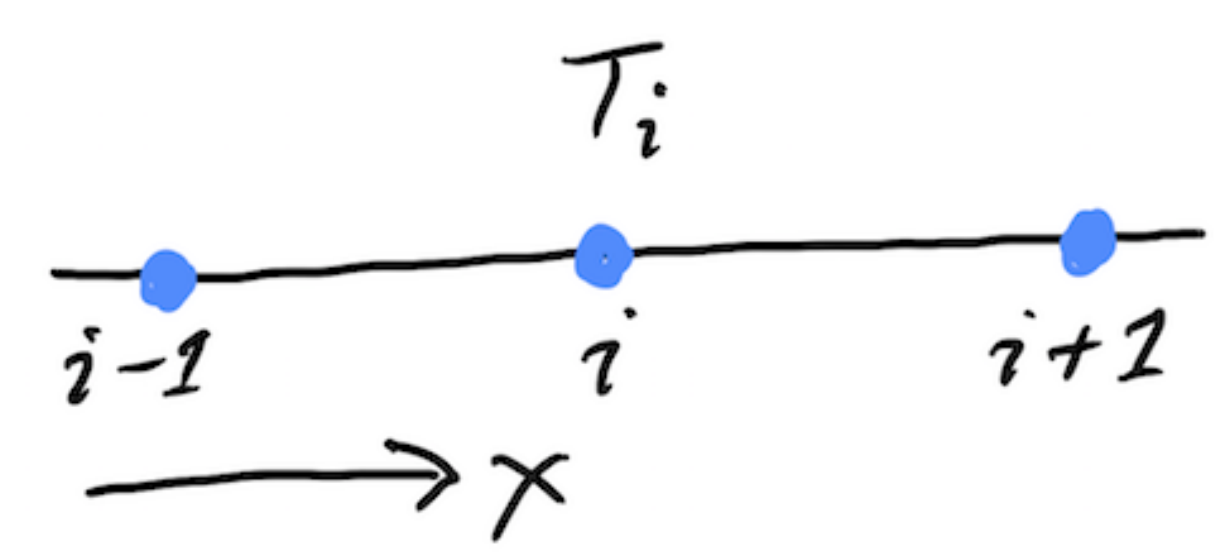
\includegraphics[scale=0.2]{pic/heatTwoway.png}
\end{center}
Now consider transient heat convection/conduction. The temperature at any given time is influenced by
existing conditions before that point \textbf{in time}. Here, \(\textbf{t}\) is a \uline{one way} coordinate for transient heat conduction/convection

\begin{center}
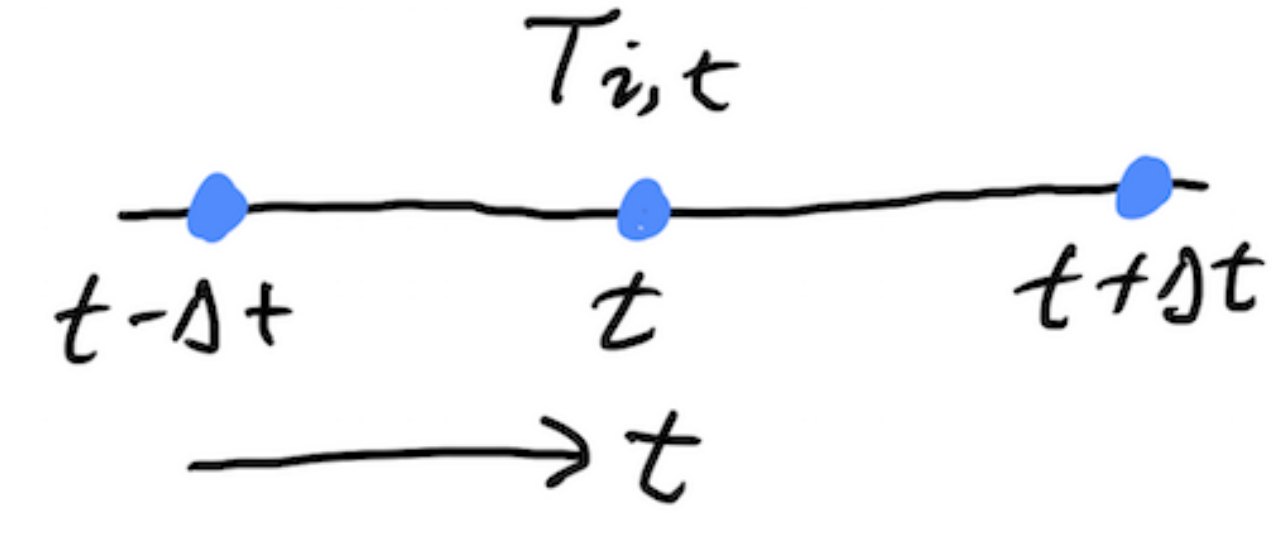
\includegraphics[scale=0.2]{pic/heatOneway.png}
\end{center}
Recall our generic conservation equation:
\begin{equation*}
\frac{\partial \phi}{\partial t} + \nabla \cdot (\textbf{u}\phi) + \nabla \cdot \textbf{J}_\phi = S_\phi
\end{equation*}
We consider the diffusion term or \textbf{elliptic PDE} :  \(\boxed{\nabla \cdot \textbf{J}_\phi}\) to be \uline{two-way in space}\\
Likewise, the convection term or \textbf{parabolic PDE} :  \(\boxed{\nabla \cdot (\textbf{u}\phi)}\) to be \uline{one-way in space} 

\subsection{Main idea behind Discretization}
\label{sec:org954e1c0}
Our goal is to:
\begin{itemize}
\item replace the PDEs' continuous solution with \uline{discrete} solution, at \uline{specific location} that approximates the continuous
solution suitably.
\end{itemize}
For finite volume:
\begin{enumerate}
\item domain is split into \uline{non overlapping finite} regions that fill the domain
\item the discrete point is at the \uline{centroid} of each control volume with volume \(V_p\), at position \(\textbf{x}_p\)
\item surround these cells, we have the "faces". At the center of these "faces", we have the integration point at position
\(\textbf{x}_{ip}\)
\item the governing equations are then integrated over a control volume, where surface flux terms and volume source terms are
balanced. 
\begin{center}
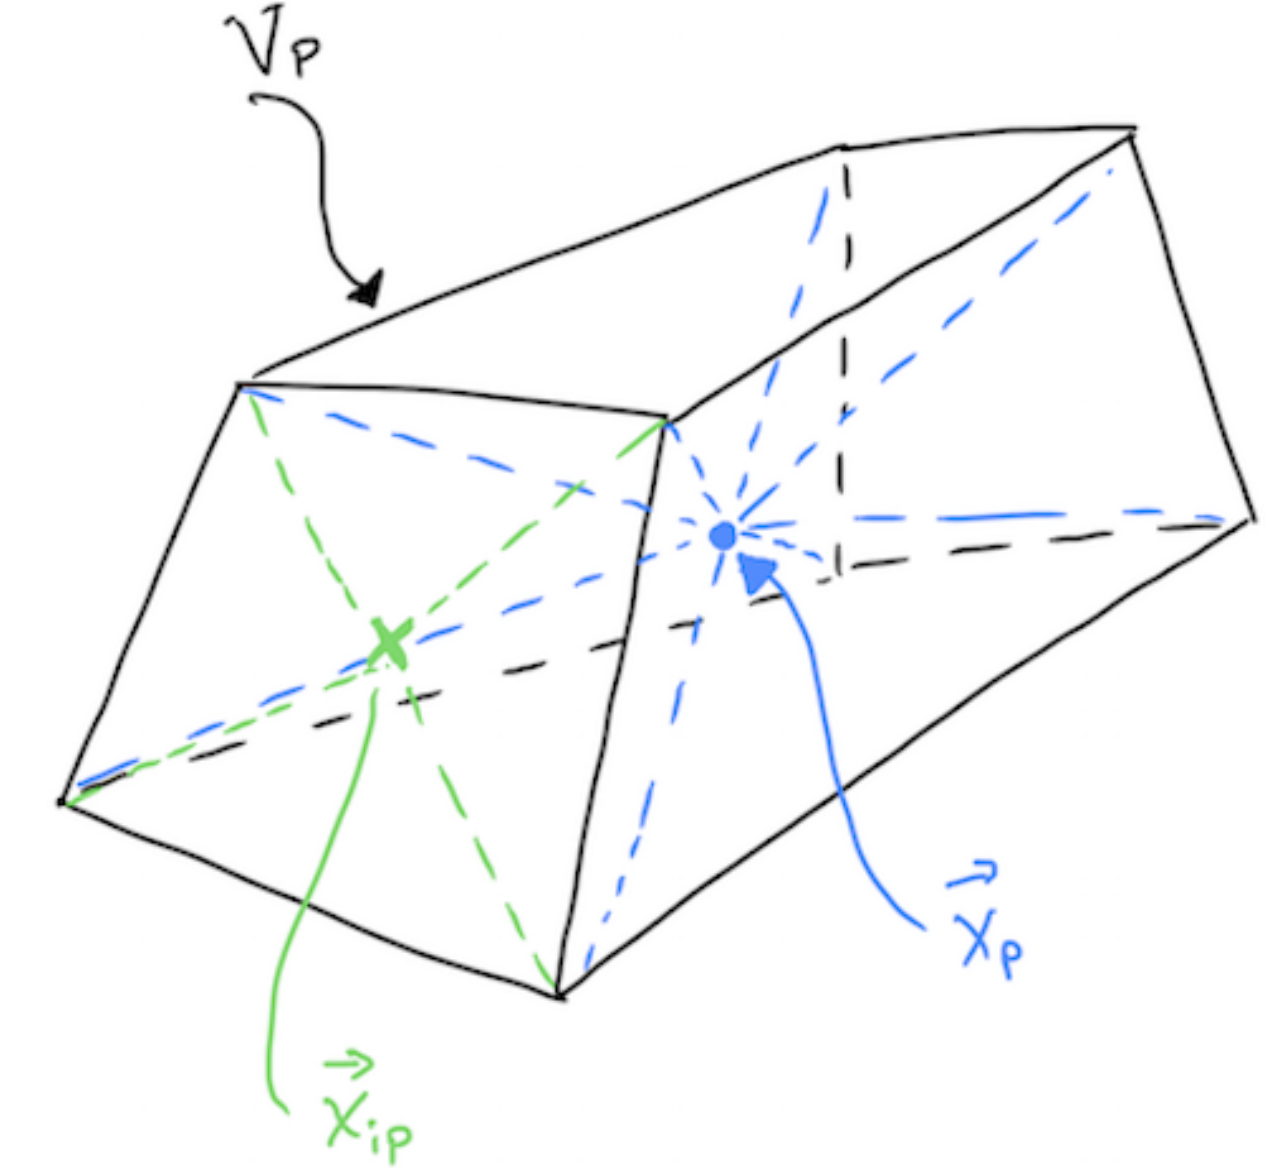
\includegraphics[scale=0.2]{pic/finiteVolumeElement.png}
\end{center}
\end{enumerate}
\subsection{Determine Cell Centre + Face Integration Points}
\label{sec:org06aca3c}
\uline{Cell centre} => location of \uline{solution} variables.\\
Points on \uline{face} => \uline{fluxes} are evaluated.\\
Consider a volume integral of a quantity \(\phi\), we may express this integral in discrete form as follow:
\begin{equation}
\int_V \phi dV \approx \phi_P V_P 
\end{equation}
where \(\phi_P\) is the value of \(\phi\) at some internal within \(V\) and \(V_P\) is total volume of the cell:
\begin{equation}
V_P = \int_V dV 
\end{equation}
To prove the above result, we expand \(\phi\) in a Taylor series about the point \(P\).
\begin{equation}
\phi \approx \phi_P + \nabla \phi_P (\textbf{x} - \textbf{x}_P) + \nabla^2 \phi_P (\textbf{x}-\textbf{x}_P)(\textbf{x}-\textbf{x}_P) + .... O(\delta^3) 
\end{equation}
with \(\delta\) being the characteristic grid spacing. Substitute this into our assumed expression for \(V_P\):
\begin{equation}
\int_V \phi dV \approx \int_V [\phi_P + \nabla \phi_P (\textbf{x} - \textbf{x}_P) + \nabla^2 \phi_P (\textbf{x}-\textbf{x}_P)(\textbf{x}-\textbf{x}_P) + .... O(\delta^3)]dV 
\end{equation}
We note that \(\phi_P\) and its derivatives are constants:
\begin{equation}
\int_V \phi dV \approx \phi_P dV + \nabla \phi_P \int_V (\textbf{x}-\textbf{x}_P) dV + \nabla^2 \phi_P \int_V (\textbf{x}-\textbf{x}_P)(\textbf{x}-\textbf{x}_P)dV + .... O(\delta^3) 
\end{equation}
Because our \(\textbf{x}_P\) point is at centroid, so \(\int_V (\textbf{x}-\textbf{x}_P) dV = 0\). Likewise, the last term is also neglected,
resulting in:
\begin{equation}
\int_V \phi dV \approx [\phi_V + O(\delta^2)]V_P
\end{equation}
This means that there is a second order error when approximating the cell volume in this way.  This is OK because the accuracy of
the method is also second order.\\
\textbf{Note}: If our \$\textbf{x}\textsubscript{P}\} does not lie at the centroid of the cell. The second term,\(\int_V (\textbf{x}-\textbf{x}_P) dV\) does not go
to zero, making our approximation to be 1st order, which is worse. 
\subsection{Transient term}
\label{sec:orge40d5a5}
Here we deal with the transient term, \(\frac{\partial \phi}{t}\). Discretization of this term relies on:
\begin{itemize}
\item order of accuracy
\item implicit vs explicit
\end{itemize}
The idea is to integrate this term over control volume \(V_P\) and some time step \(\Delta t = t_1 - t_0\) to get
the formula for the discretization.
\begin{equation}
\int_{t_0}^{t_1} \int_V \frac{\partial \phi}{\partial t}dVdt \approx (\phi V_P)^{t_1} - (\phi V_P)^{t_0} 
\end{equation}
\subsection{Advection term}
\label{sec:orge5562ae}
Here we deal with the advection term, \(\nabla \cdot (\textbf{u} \phi)\). Similar to the transient term, the formula for the
discretization can be obtained by integrating over the control volume \(V_P\). We also employ Gauss' theorem to convert
\uline{volume integral} to \uline{surface integral}:
\begin{equation}
\int_V \nabla \cdot (\textbf{u}\phi)dV = \int_S (\textbf{u}\phi) \cdot \textbf{n}dS
\end{equation}
For the surface integral, we approximate by summing up over the faces surrounding the cell, each with area \(A_{ip}\).
\begin{equation}
\int_S (\textbf{u}\phi) \cdot \textbf{n}_{ip}dS \approx \sum_{i=0}^{N_{ip}-1} \textbf{u}_{ip} \cdot \textbf{n}_{ip} \phi_{ip}A_{ip}
\end{equation}
\textbf{Note}:
\begin{itemize}
\item using C program notation, so we sum from 0 till \(N_{ip}-1\)
\item approximate \(\textbf{u}_{ip}\) by many interpolation methods
\item interpolating \(\phi_{ip}\) carefully to obtain \uline{stable} numerical method.
\end{itemize}
\subsection{Diffusion term}
\label{sec:org5771962}
Now, we deal with the diffusion term, \(\nabla \cdot \textbf{J}_\phi\). Similar to the advection term, we integrate over a control
volume, then apply Gauss' theorem
\begin{equation}
\int_V \nabla \cdot \textbf{J}_\phi dV = \int_S \textbf{J}_\phi \cdot \textbf{n}dS
\end{equation}
Again, the surface integral is approximated as discrete sum over the faces surrounding the cell:
\begin{equation}
\int_S \textbf{J}_\phi \cdot \textbf{n}dS \approx \sum_{i=0}^{N_{ip}-1} \textbf{J}_{\phi, ip} \cdot \textbf{n}_{ip}\textbf{A}_{ip}
\end{equation}
where the flux, \(\textbf{J}_{\phi,ip}\) is interpolated from neighboring cell values. 
\subsection{Source term}
\label{sec:orge080544}
Recall our source term: \(S_\phi\), we assume that the source term is \uline{piecewise continuous}, with one specific value, \(S_\phi\),
being represented by each cell. We can then write:
\begin{equation}
\int_V S_\phi dV \approx S_\phi V_P
\end{equation}
Generally, the source term may depend on \(\phi\) so linearization is needed to obtain \uline{stable} numerical method. 
\subsection{Linearization}
\label{sec:org60cde72}
With regard to our last point about \(J_\phi\), the discretized terms depend non linearly on the solution. This non-linearity
is caused by:
\begin{itemize}
\item source term depend non linearly on primitive variable, e.g. \(J_\phi\).
\item non linearities in the governing equation, e.g. advection term \(\nabla \cdot (\textbf{u} \phi)\)
\item on non-orthogonal grid, gradient correction terms are needed <= these are non linear.
\end{itemize}
To linearize, we assume the governing PDE is represented by the following general differential operator
\begin{equation}
L(\phi^*) = 0
\end{equation}
where:\\
\begin{itemize}
\item \(\phi^*\) = the continuous solution to the PDE
\item Note that to solve a PDE using finite volume, the continuous solution \(\phi^*\) is approximated by the discrete solution vector
\(\phi \in \mathbb{R}\) on \(N\) number of control volume. Our PDE is then integrated over each control volume and each term in the
governing equation is approximated using the discrete solution \(\phi\)
\item Of course, the numerical solution will not satisfy the discretized equation exactly; rather we will have a residual,
\(\textbf{r} \in \mathbb{R}^N\).
\end{itemize}
We expand the residual about the solution \(\phi_i\) at iteration \(i\), and find the solution where \(r = 0\):
\begin{equation}
\textbf{r}(\phi_i) + \left. \frac{\partial \textbf{r}}{\partial \phi}\right|_{\phi_i}(\phi - \phi_i) = 0
\end{equation}
We define the \textbf{Jacobian of the residual vector} as:
\begin{equation}
\textbf{J}(\phi) = \frac{\partial \textbf{r}}{\partial \phi}
\end{equation}
We use this to update according to fix point iteration:
\begin{equation}
\phi = \phi_i + \Delta \phi_i
\end{equation}
where:
\begin{equation}
\Delta \phi = (\phi - \phi_i)
\end{equation}
and:
\begin{equation}
\textbf{J}(\phi_i)\Delta \phi = -\textbf{r}(\phi_i)
\end{equation}
The remaining unknowns are: the residual vector \(\textbf{r}\) and Jacobian matrix \(\textbf{J}(\phi_i)\).\\
\textbf{Note}: we can express the linear system for a control volume P as:
\begin{equation}
a_P\delta \phi_P + \sum_{nb} a_{nb}\delta \phi_{nb} = -r_P
\end{equation}
where \(nb\) is sum over all neighboring cells.  The coefficients are defined as:
\begin{align}
a_P &= \frac{\partial r_P}{\partial \phi_P}\\
a_{nb} &= \frac{\partial r_P}{\partial \phi_{nb}}
\end{align}
\subsection{Four Basic Rules}
\label{sec:orgaada041}
Outlined by Patankar(1980), these 4 rules are:
\begin{itemize}
\item \textbf{Rule 1: Consistency at control volume faces\\
}
For common faces between cells, the flux through those common faces must be the same when evaluated at each cell.
If this is not the case, then it means there is an artificial source of the energy at the face.
\item \textbf{Rule 2: \(\alpha_p > 0\) and \(\alpha_{nb} < 0\)}\\
Consider situations involving only convection and diffusion and all other conditions unchanged: if \(\phi\) in 1 cell
increases, then we can expect \(\phi\) in the neighboring cells to increase as well. The only way that this could happen is in this equation
\begin{equation*}
a_P\delta \phi_P + \sum_{nb} a_{nb}\delta \phi_{nb} = -r_P
\end{equation*}
\(a_p\) must have opposite sign from each of its \(a_{nb}\) coefficients, just so that \(\delta \phi_p\) and \(\delta \phi_{nb}\)
have the same signs and \(r_p\) is unchanged.
\item \textbf{Rule 3: Negative slope linearization of source terms}\\
Suppose we have a source term in the form: \(S_\phi = a + b\phi_P\). If this is moved to the LHS, the coefficient \(a_P\) can be negative
if \(b\) is positive. So we require that \(b < 0\), or negative slope linearization. The idea is that a positive slope linearization would be
unstable because the source would cause the variables to increase, which would then increase the source term. This would continue indefinitely
and without bounds. In terms of heat transfer, we can have a heat source that grows with temperature and also a heat sink for removal of temperature.
This is done to avoid an uncontrolled increase in temperature.
\item \textbf{Rule 4: Sum of neighboring coefficients}\\
Our governing equations contain derivatives of dependent variables, i.e. both \(\phi\) and \(\phi+c\) will satisfy the same governing equations.
Thinking practically, this means that temperature field in both Kelvin and Celcius would both satisfy the same discretized equations, because Celcius and Kelvin
scale are related via a constant.  For this to be true, we require:
\begin{equation*}
a_p = - \sum_{nb} a_{nb}
\end{equation*}
Note that in the case of the linearization of the source term above, it indicates that same equation cannot be used for both \(\phi\)
and \(\phi+c\). So in this case, make sure to modify the source term coefficients appropriately.
\end{itemize}
\clearpage
\section{STEADY DIFFUSION EQUATION}
\label{sec:org0867f57}
\subsection{Problem Definition}
\label{sec:org262ce8c}
We consider the solution of a \uline{steady}, \uline{1D} heat diffusion equation
\begin{equation}
-k \nabla^2 T - S = 0
\end{equation}
\subsection{Discretization}
\label{sec:org54dbf93}
Recall our diffusion term can be discretized as:
\begin{equation}
\int_S \textbf{J} \cdot \textbf{n} dS \approx \sum_{i=0}^{N_{ip}-1} \textbf{J}_{ip}\cdot \textbf{n}_{ip}A_{ip}
\end{equation}
Our flux \(\textbf{J}\) here is the \uline{diffusive} flux, so: \(\textbf{J} = -k \nabla T\). Thus:
\begin{equation}
\int_S \textbf{J} \cdot \textbf{n} dS \approx -\sum_{i=0}^{N_{ip}-1} k_{ip} \nabla T_{ip}  \cdot \textbf{n}_{ip}A_{ip}
\end{equation}
We assume constant thermal conductivity, \(k_{ip} = k\). A 1D control volume, with West/East faces and unit vectors drawn, is shown below:
\begin{center}
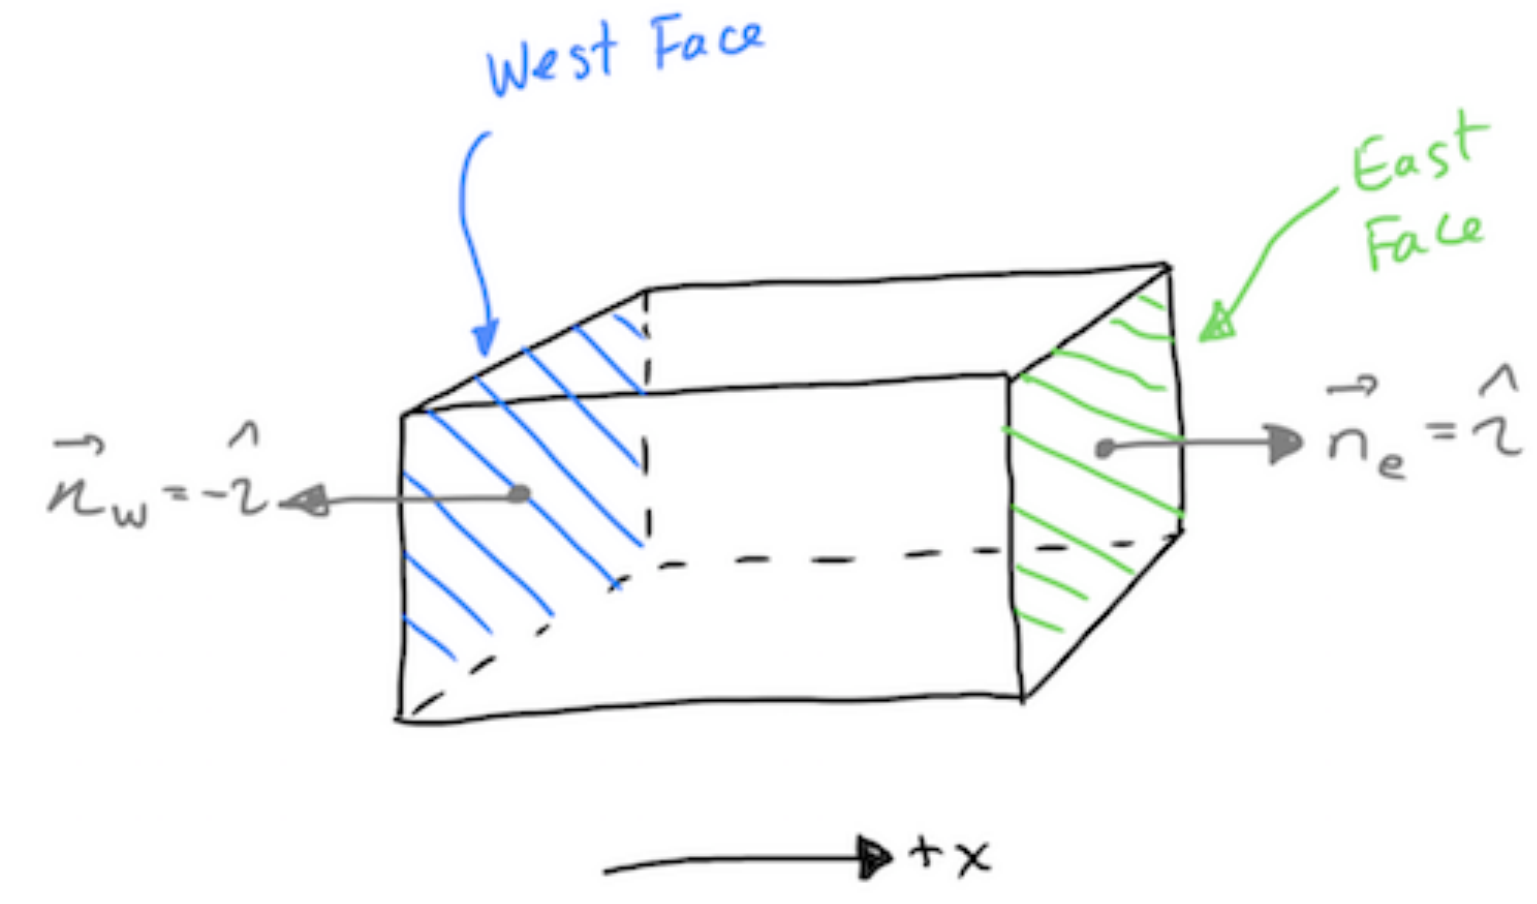
\includegraphics[scale=0.2]{pic/heat1D_CV.png}
\end{center}
Since we are in 1D, our unit vector is in the \(\textbf{i}\) only.\\
Thus, \(\nabla T \cdot \textbf{n} = \nabla T \cdot \textbf{i}\).\\
But, \(\nabla T \cdot \textbf{i} = \left < \frac{\partial T}{\partial x} \textbf{i} + \frac{\partial T}{\partial y} \textbf{j} + \frac{\partial T}{\partial z} \textbf{k}
  \right > \cdot \left <1 \textbf{i} + 0 \textbf{j} + 0 \textbf{k}    \right> = \frac{\partial T}{\partial x}\). \\
With these points in mind, the discretization for the diffusion term is simplified to:
\begin{equation}
\int_S \textbf{J} \cdot \textbf{n} dS \approx k \left .\frac{\partial T}{\partial x}\right|_w A_w
- k \left .\frac{\partial T}{\partial x}\right|_e A_e 
\end{equation}
The diagram below shows the cell locations and the nomenclature for the distance between them, note how \(\Delta x\) is center-center
\begin{center}
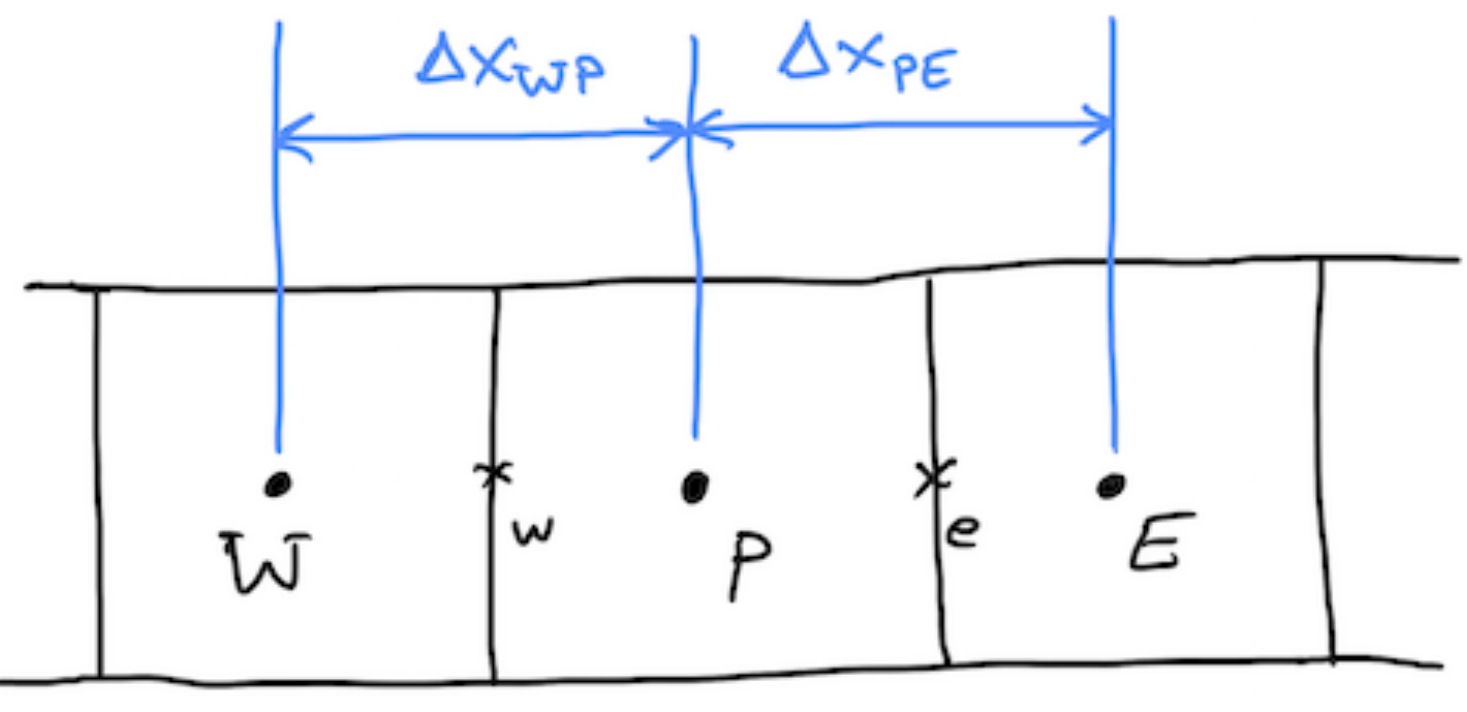
\includegraphics[scale=0.2]{pic/heat1D_cell.png}
\end{center}
We apply \uline{finite differences} to the derivatives in the diffusion term, i.e.:
\begin{equation}
k \left .\frac{\partial T}{\partial x}\right|_w A_w - k \left .\frac{\partial T}{\partial x}\right|_e A_e
= k\frac{T_P-T_W}{\Delta x_{WP}}A_w - k\frac{T_E-T_P}{\Delta x_{PE}}A_e
\end{equation}
Our discretized source term is simply:
\begin{equation}
\int_V SdV \approx S_PV_P
\end{equation}
where \(S_P\) = value of source term \textbf{within} the cell, and \(V_P\) = cell volume.\\
Put everything on one side, we can form the \uline{residual equation} for the cell \(\textbf{P}\) as:
\begin{equation}
r_P = - k\frac{T_E-T_P}{\Delta x_{PE}}A_e + k\frac{T_P-T_W}{\Delta x_{WP}}A_w - S_PV_P
\end{equation}
or expressing in terms of the diffusive fluxes, \(\textbf{F}^d\), through each face:
\begin{equation}
r_P = F_{e}^d - F_{w}^d - S_PV_P
\end{equation}
where:\\
\begin{alignat}{2}
F_{e}^d &= - k\frac{T_E-T_P}{\Delta x_{PE}}A_e &&= -D_e(T_E- T_P)\\
F_{w}^d &= - k\frac{T_P-T_W}{\Delta x_{WP}}A_w &&= -D_w(T_P- T_W)\\
D_e &= \frac{kA_e}{\Delta x_{PE}}\\
D_w &= \frac{kA_w}{\Delta x_{WP}}
\end{alignat}
Our cell residual equation is then:
\begin{equation}
r_P = D_w (T_P-T_W)-D_e(T_E-T_P)-S_PV_P
\end{equation}
The linearized coefficients are then calculated as:
\begin{align}
a_P &= \frac{\partial r_P}{\partial T_P} = D_w + D_e - \frac{\partial S_P}{\partial T_P}V_P\\
a_W &= \frac{\partial r_P}{\partial T_W} = -D_w\\
a_E &= \frac{\partial r_P}{\partial T_E} = -D_e
\end{align}
Recall that we can form an algebraic system of equation for each control volume like this:
\begin{align}
a_P\delta \phi_P + \sum_{nb} a_{nb}\delta \phi_{nb} &= -r_P\\
a_P\delta T_P + a_W\delta T_W + a_E \delta T_E &= -r_P 
\end{align}
The above linear system of equations can be written as as tridiagonal matrix, like this:
\begin{center}
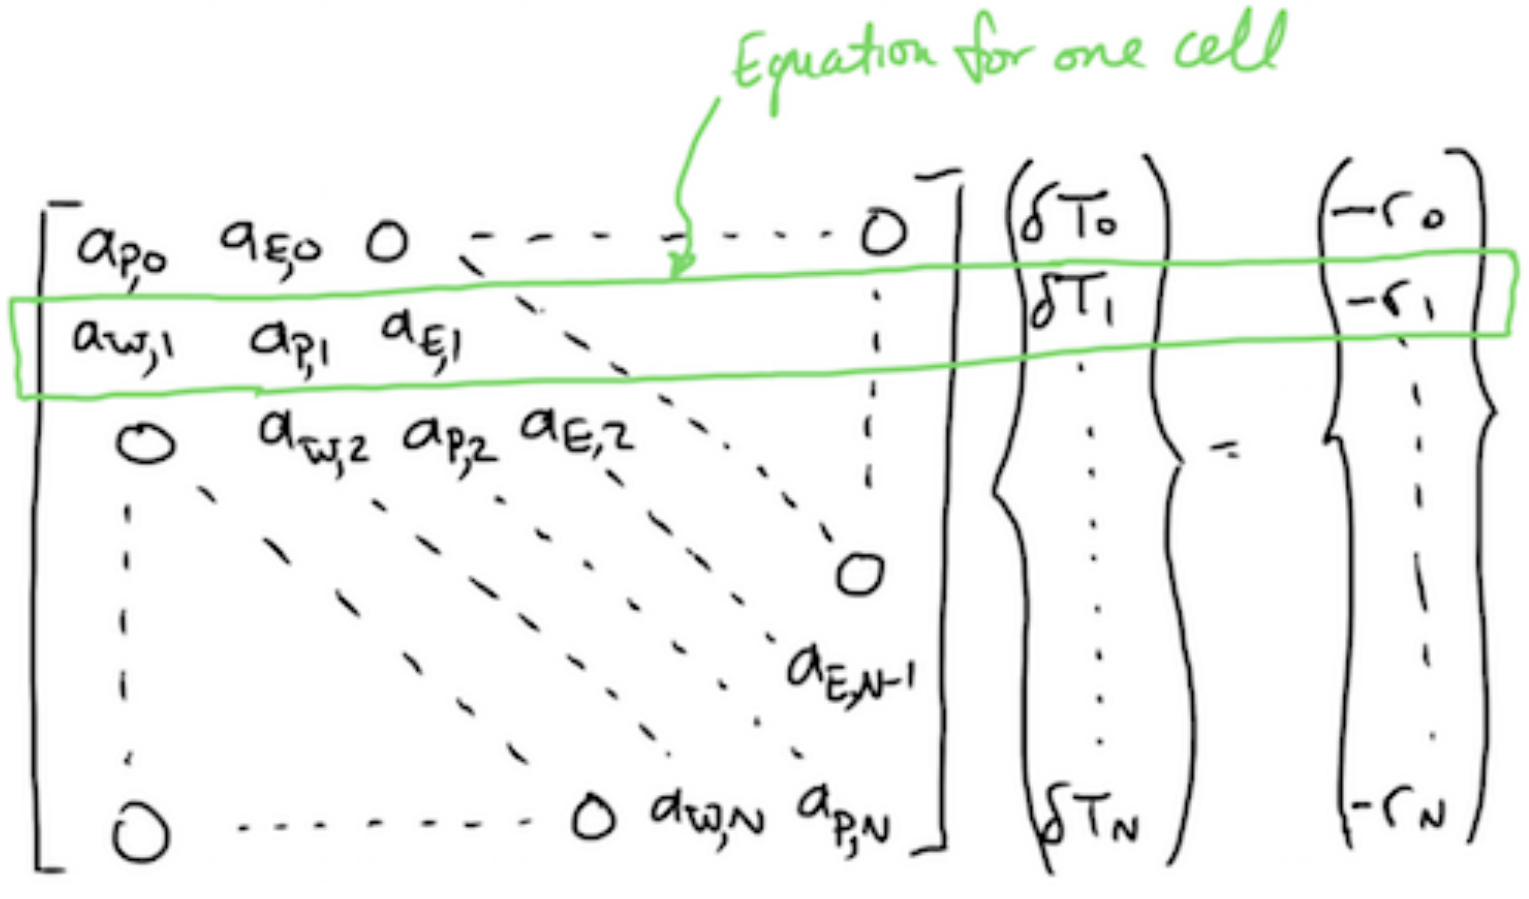
\includegraphics[scale=0.2]{pic/heat1D_tridiagonal.png}
\end{center}
\textbf{Note}: The first and last row only has 2 non zero elements each. This is because these are the left most/right most side and they are
adjacent to the domain boundary. Therefore, special \uline{boundary conditions} are needed to be set. \\
In matrix notation, we are solving:
\begin{equation}
\textbf{A}\textbf{x} = \textbf{b}  
\end{equation}
where \(\textbf{A}\) is the Jacobian matrix, \(\textbf{b} = \textbf{-r}\) is the residual vector, \(\textbf{x} = \delta \textbf{T}\)
is the solution correction. At each current iteration \(i\), the solution is updated according to:
\begin{equation}
\textbf{T} = \textbf{T}_i + \delta \textbf{T}i
\end{equation}
\subsection{Source Terms}
\label{sec:org4329de6}
Our source term can have many forms, depending on the type of heat source. We will assume \emph{external convection}
and \emph{radiation exchange}:
\begin{itemize}
\item For external convection:
\begin{equation}
\frac{S_{conv,P}}{V_P} = -hA_0(T_P-T_{\infty,c})
\end{equation}
where:
\begin{itemize}
\item \(h\) is the convective coefficient.
\item \(A_0\) is external surface area of the cell \(P\).
\item \(T_P\) is temperature at the centroid of cell \(P\).
\item \(T_{\infty,c}\) is the ambient temperature for the convection process.
\end{itemize}
\item For radiation exchange:
\begin{equation}
\frac{S_{rad}}{V_P} = -\epsilon \sigma A_0(T_P^4 - T_{\infty,r}^4)
\end{equation}
where:
\begin{itemize}
\item \(\epsilon\) is the surface emissivity.
\item \(\sigma\) is the Stefan-Boltzmann constant.
\item \(T_{\infty,r}\) is the surrounding temperature for radiation exchange.
\end{itemize}
\end{itemize}
\subsection{Discussion of Discretization Procedure}
\label{sec:org8c40f7a}
\subsubsection{Temperature Profile Assumptions}
\label{sec:orgc13581a}
When computing the diffusive fluxes through the faces, we assumed a \textbf{piecewise-linear profile} for the temperature.
This ensures that the derivatives are defined at the integration points and provides consistency for flux
at control-volume faces. For the source term, \textbf{piece-wise constant profile} is used, implying a single value of the source
term in each cell. Note that for piece-wise constant profile, the derivatives are not defined at integration points, due to
jump discontinuity. So if fluxes will be inconsistent if piecewise-constant profile is used for temperature.
\begin{center}
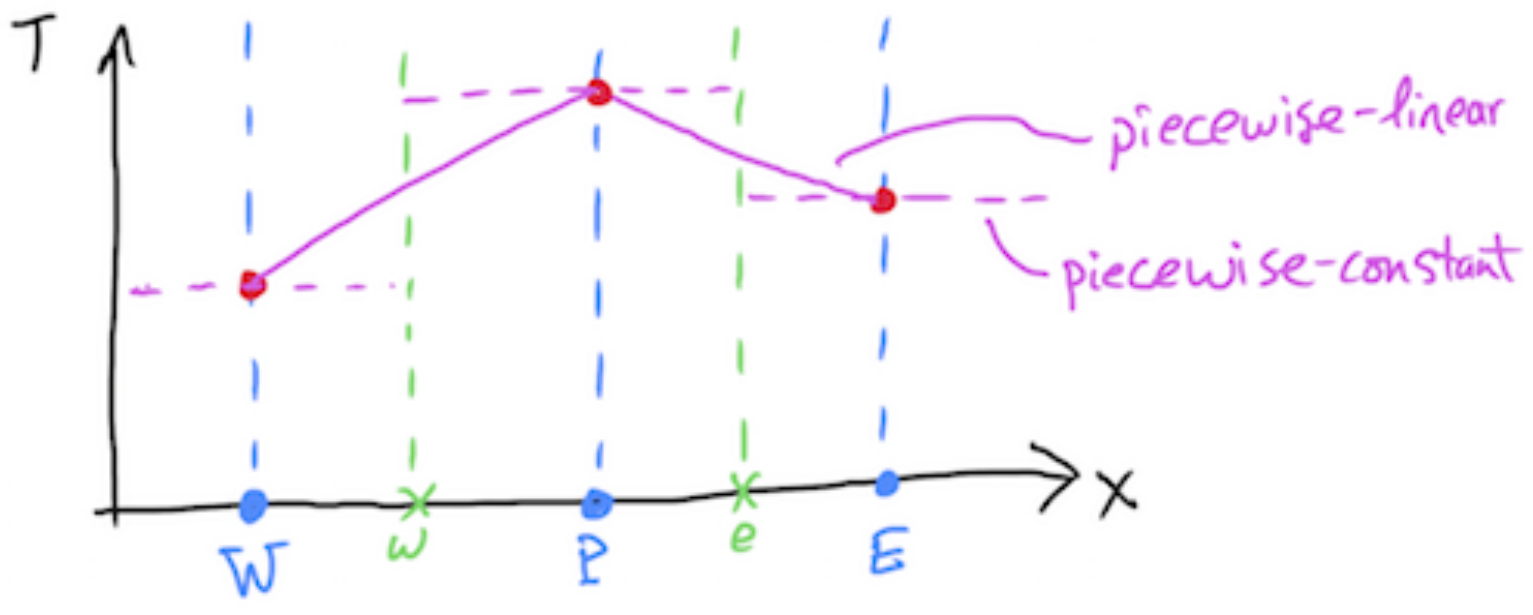
\includegraphics[scale=0.2]{pic/heat1D_profilePW.png}
\end{center}
\subsubsection{Implementation of Linearization}
\label{sec:org6649df2}
In Patakar's method, the solution of the linear system \textbf{is} the solution for the variables at the control volume center.\\
In our method, the solution of the linear system is the \textbf{correction} to apply to the previous iteration of the solution. \\
The correction method is preferred because:
\begin{itemize}
\item at convergence, the solution for the correction goes to zero \(\rightarrow\) zero a good initial guess for the linear solver.
\item linear system involves the residual vector. In Patankar's, there are more work to calculate the residual vector.
\end{itemize}
\subsubsection{Properties of the Discrete Algebraic Equations}
\label{sec:org5626a91}
Recall our algebraic equation for the linear system
\begin{equation}
a_P\delta T_P + a_W\delta T_W + a_E \delta T_E = -r_P 
\end{equation}
In Rule 2, we require that \(a_P > 0\) and \(a_W, a_E < 0\). The reason for this is if we consider the case with no source,
and the solution converge, \(r_P \rightarrow 0\):
\begin{equation}
a_P\delta T_P = -a_W\delta T_W - a_E \delta T_E  
\end{equation}
Now, suppose both \(T_P\) and \(T_E\) are pertubed.  If either of these temperatures were to rise, then \(T_P\) would also rise.
Similarly, if either temperatures were to drop, \(T_P\) should also drop. Therefore, to ensure correct physical effect, if
\(a_P > 0\) then \(a_W, a_E > 0\).\\
Consider the two cells (\(P\) and \(E\)) below:
\begin{center}
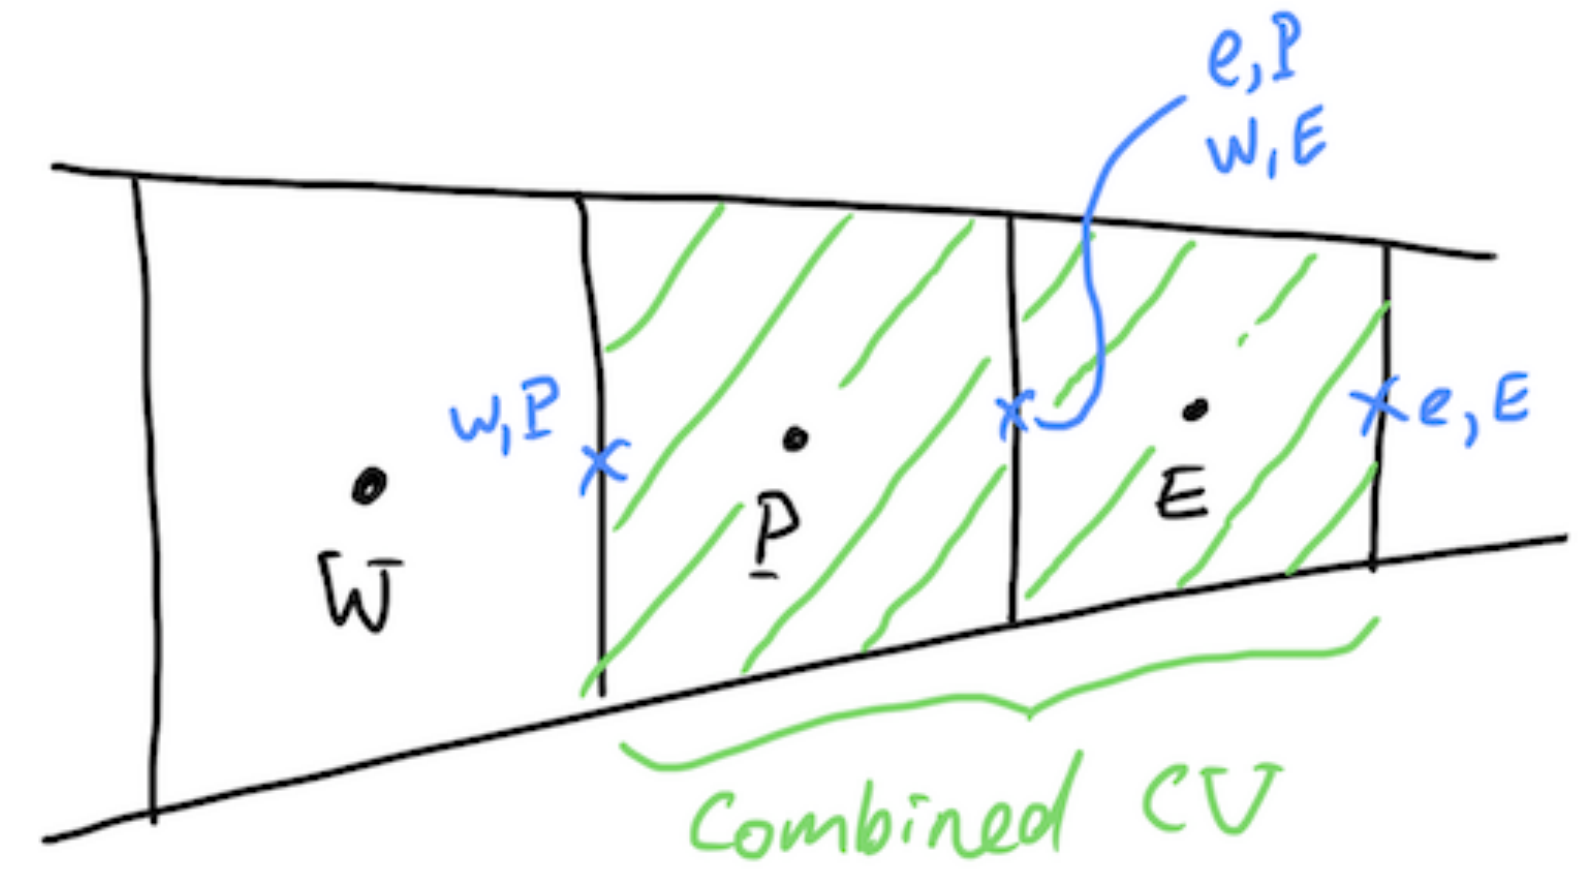
\includegraphics[scale=0.2]{pic/heat1D_cell_combined.png}
\end{center}
At convergence, \(r_P = 0\), the equation for the control volume \(P\) is:
\begin{equation}
F_{e,P}^d - F_{w,P}^d - S_PV_P = 0
\end{equation}
For the control volume \(E\):
\begin{equation}
F_{e,E}^d - F_{w,E}^d - S_EV_E = 0
\end{equation}
Adding these equations together gives:
\begin{equation}
F_{e,P}^d - F_{w,P}^d +  F_{e,E}^d - F_{w,E}^d- S_PV_P - S_EV_E = 0
\end{equation}
Note that \(F_{e,P}^d = F_{w,E}^d\) by continuity, i.e. the flux at cell \(P\) going eastward should be the same flux going
from westward at cell \(E\). If these are not equal, then it implies that there is a fictuous force at the face, which is
not reasonable. Therefore, our algebraic equation for control volume \(P\) and \(E\) becomes:
\begin{equation}
 F_{e,E}^d - F_{w,P}^d - S_PV_P - S_EV_E = 0
\end{equation}
The above equation demonstrates integral conservation: a balance of the total source term within the combined control volume with
the net diffusive flux from that same control volume. In addition, recall the definition of the diffusive flux:
\begin{align}
F_{e,P}^d &= -k \frac{T_E-T_P}{\Delta x_{PE}} A_{e,P}\\
F_{w,E}^d &= -k \frac{T_E-T_P}{\Delta x_{PE}} A_{w,E}
\end{align}
From the gemeotry of the grid, \(A_{e,P} = A_{w,E}\); therefore, it is in fact the two-point finite difference estimation of the
derivative that cause the fluxes to be equal. This is also due to the piecewise-linear profile that we assume. If we assume a
\textbf{parabolic profile} instead, there is no guarantee that the fluxes would be equal. Instead, we would have:
\begin{align}
F_{e,P}^d &= f(T_W, T_P, T_E)\\
F_{w,E}^d &= f(T_P, T_E, T_{EE})
\end{align}
This means that the flux through the common face depends on different temperature, so we cannot be sure that the derivative from either
side is consistent. 
\begin{center}
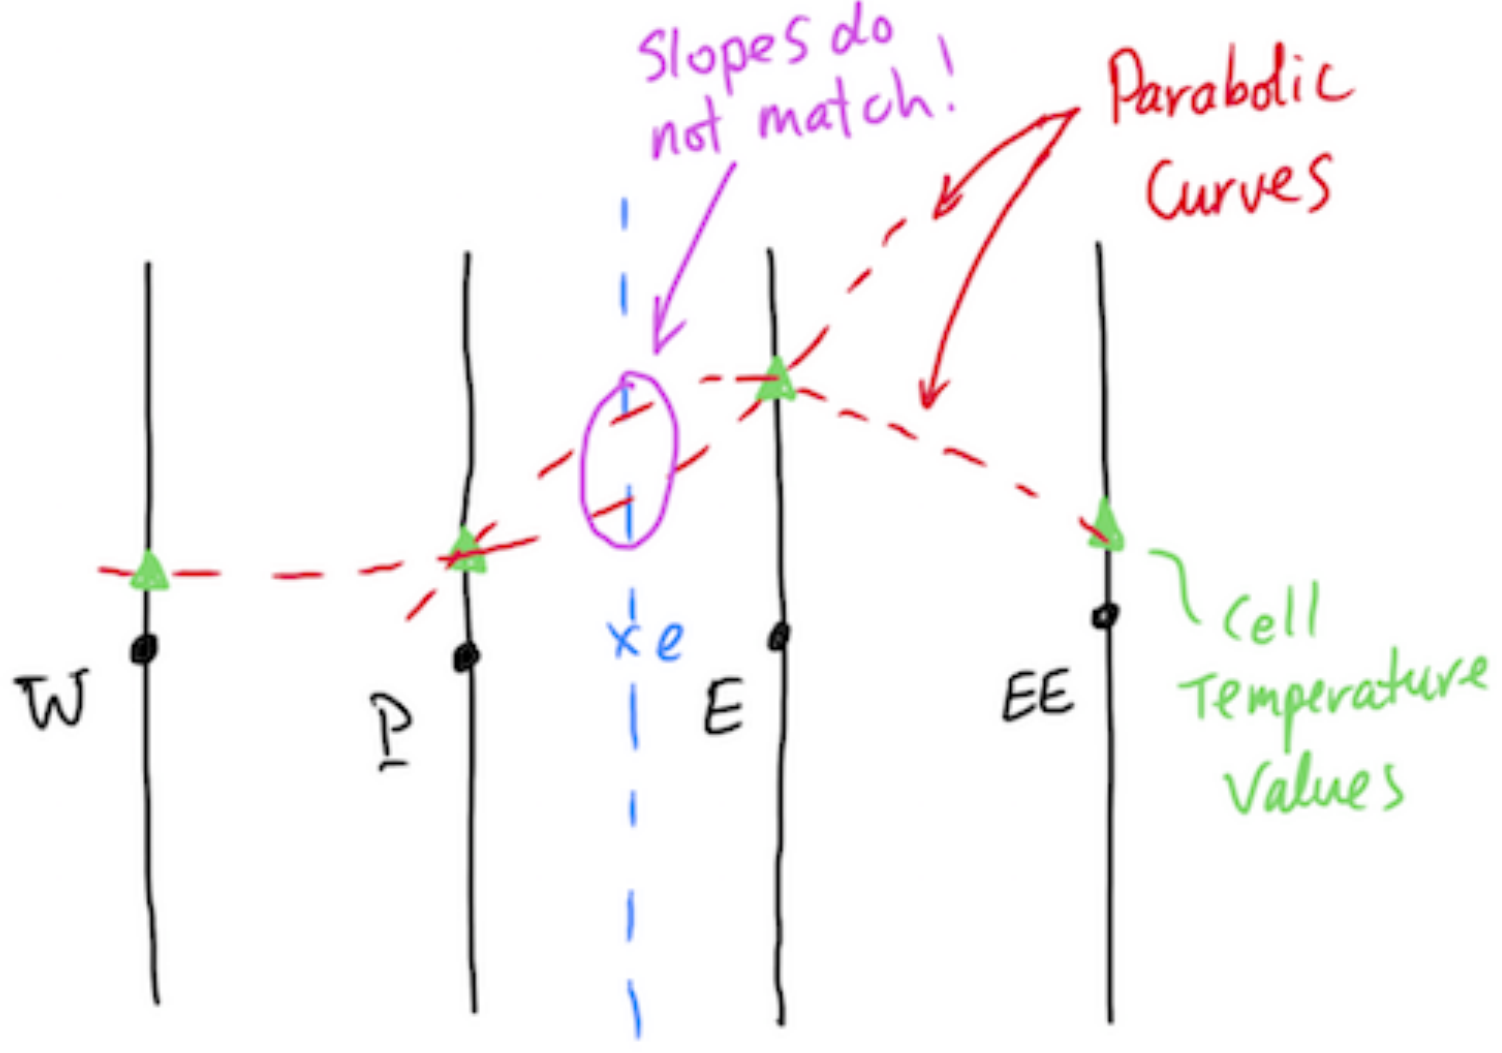
\includegraphics[scale=0.2]{pic/heat1D_profilePARABOLIC.png}
\end{center}
\subsection{Implemenation: \href{1D\_heat\_diffusion\_steady.py}{Python Code}}
\label{sec:orgdf936fd}
\lstinputlisting[language=Python]{1D_heat_diffusion_steady.py}
\section{TRANSIENT 1D HEAT DIFFUSION}
\label{sec:orgb6ea20a}
\subsection{Problem Definition}
\label{sec:orged12f0f}
In contrast to the steady case, here we are solving the following transient 1D heat diffusion equation
\begin{equation}
\frac{\partial (\rho c_p T)}{\partial t} = k \nabla^2 T + S
\end{equation}
assuming constant \(\rho\) and \(c_p\)
\subsection{Discretization}
\label{sec:orgc37e5a8}
Integrating the governing equation through space and time yields:
\begin{equation}
\int_{t_0}^{t_1} \int_{V} \frac{(\partial \rho c_p T)}{\partial t} dt dV = \int_{t_0}^{t_1} \int_{V} k \nabla^2 T dt dV + \int_{t_0}^{t_1} \int_{V} S dt dV
\end{equation}
By assuming a timestep \(\Delta t = t_1 - t_0\), we also assume that the solution is stored at time levels \(t\) and later at \(t + \Delta t\). Thus, we can assume various profiles for the integrands as functions of time.  Here, we will examine the following:
\begin{itemize}
\item \textbf{Fully explicit}: evaluate the integrands on RHS at initial time level, \(t_0 = t\).
\item \textbf{Fully implicit}: evaluate the integrands on RHS at final time level, \(t_1 = t_0 + \Delta t\)
\item \textbf{Crank Nicolson}: assume a linear profile of the RHS over the interval \(\Delta t\).
\end{itemize}
For the LHS, we interchange the order of integration, which results in this, for a control volume \(\textbf{P}\):
\begin{equation}
\int_{t_0}^{t_1} \int_{V} \frac{(\partial \rho c_p T)}{\partial t} dt dV = (\rho c_p T_p)^{t+\Delta t} - (\rho c_p T_p)^t 
\end{equation}
Recall that for the steady case, the diffusive term is the difference in flux. Here, we add a weighting function \(w\) to control the assumed variation of the integrand over the timestep. 
 \begin{equation}
\int_{t_0}^{t_1} \int_{V} k \nabla^2 T dt dV = -\left [\omega(F_e^d)^{t + \Delta t} + (1-\omega)(F_e^d)^t \right ]\Delta t +
\left [\omega(F_w^d)^{t + \Delta t} + (1-\omega)(F_w^d)^t \right ]\Delta t
\end{equation}
\begin{center}
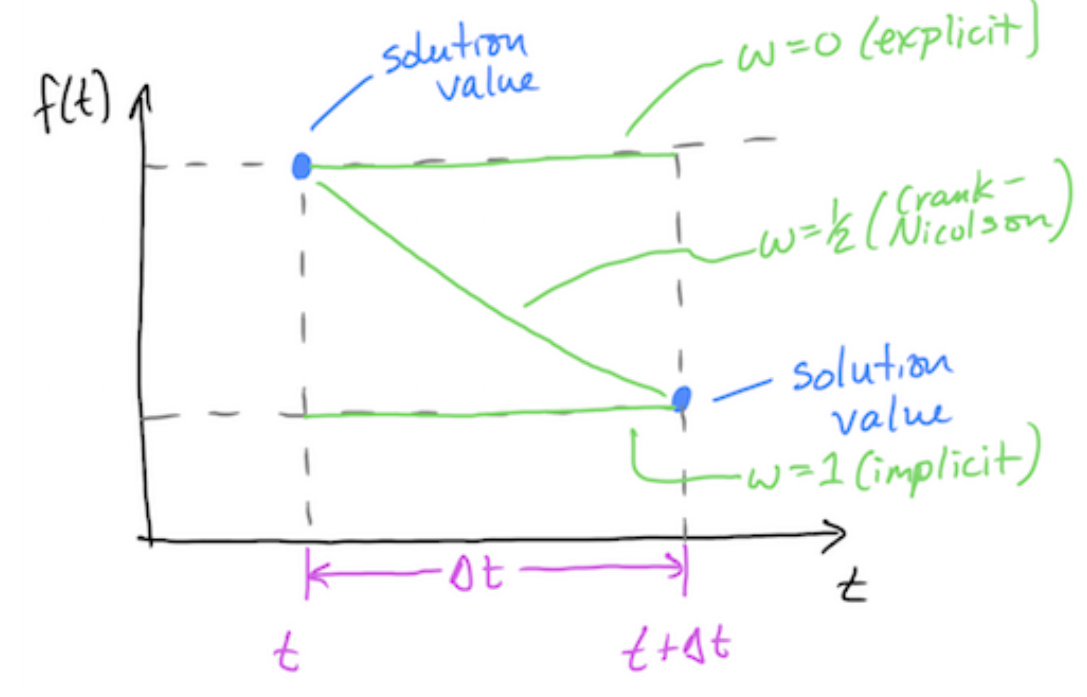
\includegraphics[scale=0.3]{pic/transientHeat_omega.png}
\end{center}
Grouping the time levels together:
\begin{equation}
 \int_{t_0}^{t_1} \int_{V} k \nabla^2 T dt dV = \left[\omega[F_w^d-F_e^d \right ]^{t+\Delta t}\Delta t +
 (1-\omega)\left [F_w^d - F_e^d \right ]^t\Delta t
\end{equation}
Assuming no source term, \(S = 0\), constant properties and divide by \(\Delta t\), our discretized equation becomes
 \begin{equation}
\rho c_p \frac{T_P^{t+\Delta t} - T_P^t}{\Delta t} V_P = \omega \left[F_w^d-F_e^d \right ]^{t+\Delta t} +
  (1-\omega)\left [F_w^d - F_e^d \right ]^t\
 \end{equation}
\textbf{\uline{Note}}
\begin{itemize}
\item fully implicit and fully explicit are \emph{1st order} accurate in time.
\item Crank-Nicolson are \emph{2nd order} accurate in time.
\begin{itemize}
\item but Crank-Nicolson are \emph{less stable}, cause oscillations.
\end{itemize}
\item Generally, explicit solutions do not require the solution of a system of equations. All diffusive fluxes are calculated using solution values from previous timestep
\item Implicit requires solution of a linear system at current time step. The same is true for Crank-Nicolson, or any scheme where \(0<\omega < 1\)
\end{itemize}
\subsection{Analysis of Explicit Scheme}
\label{sec:org21fc8cb}
Recall explicit scheme means \(\omega = 0\). Our discretized equation becomes:
\begin{equation}
\rho c_p \frac{T_P ^{t+\Delta t}}{\Delta t} V_P = [F_w^d-F_e^d]^t + \rho c_p \frac{T_P^t}{\Delta t}V_P 
\end{equation}
Recall that the fluxes can be defined as:
\begin{alignat}{2}
F_{e}^d &= - k\frac{T_E-T_P}{\Delta x_{PE}}A_e &&= -D_e(T_E- T_P)\\
F_{w}^d &= - k\frac{T_P-T_W}{\Delta x_{WP}}A_w &&= -D_w(T_P- T_W)\\
D_e &= \frac{kA_e}{\Delta x_{PE}}\\
D_w &= \frac{kA_w}{\Delta x_{WP}}
\end{alignat}
Thus, our explicit formulation becomes:
\begin{equation}
\rho c_p \frac{T_P ^{t+\Delta t}}{\Delta t} V_P = D_eT_E^t + D_wT_W^t + \left ( \frac{\rho c_p V_P}{\Delta t} - D_e - D_w \right)T_P^t 
\end{equation}
To get correct physical influence, the coefficient of \(T_P^t\) must be positive, to ensure \(\uparrow T_P^t\) leads to \(\uparrow T_P^{t+\Delta t}\).
Therefore, our timestep must be selected such that:
\begin{equation*}
\frac{\rho c_p V_P}{\Delta t} \geq D_e + D_w 
\end{equation*}
or
\begin{equation*}
\Delta t \leq \frac{\rho c_p V_P}{D_e + D_w} = \frac{1}{\frac{D_e}{\rho c_p V_P} + \frac{D_w}{\rho c_p V_P} }
\end{equation*}
Simplifying further, we assume \(V_P = A\Delta x\) where \(A\) is the cross-sectional area of the domain at \(P\), and \(\Delta x\) is the grid spacing.
Also assuming \(A_e, A_w \approx A\)
\begin{equation*}
\frac{D_e}{\rho c_p V_P} \approx \frac{\frac{kA_e}{\Delta x}}{\rho c_p A \Delta x} = \frac{k}{\rho c_p}\frac{1}{\Delta x^2} = \frac{\alpha}{\Delta x^2}
\end{equation*}
The quantity \(\frac{\Delta x^2}{\alpha}\) may be interpreted as the timescale associated with conduction through the face.\\
For uniform grid, \(A_e =
   A_w = A\), the timestep restriction is:
\begin{equation}
\Delta t \leq \frac{1}{\frac{\alpha}{\Delta x^2} + \frac{\alpha}{\Delta x^2}} = \frac{\Delta x^2}{2\alpha}
\end{equation}
Note how our timestep is related to the square of the grid size, so the a fine grid will have a very small "\(\Delta x^2\)".
To study this, we consider an iron bar with \(\alpha = 23.1 \times 10^{-6}\) [\(m^2/s\)] at various grid sizes:
\begin{table}[htbp]
\label{tab:org9e0905a}
\centering
\begin{tabular}{rr}
\hline
GRID SIZE [m] & TIME STEP [sec]\\
\hline
0.01 & 2.1645022\\
0.001 & 0.021645022\\
0.0001 & 2.1645022e-4\\
0.00001 & 2.1645022e-6\\
\hline
\end{tabular}
\end{table}
\begin{center}
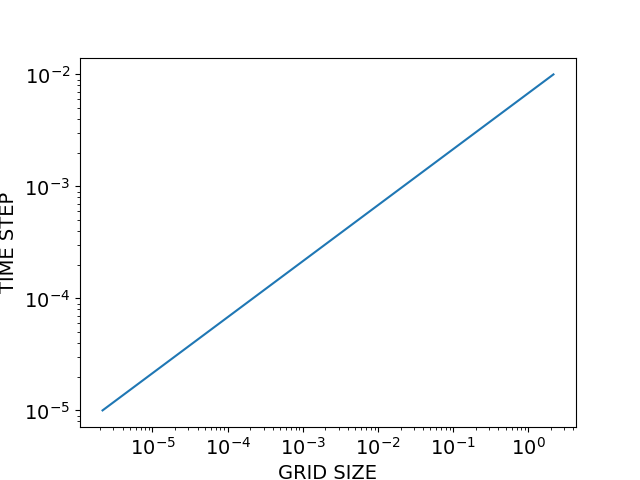
\includegraphics[scale=0.6]{pic/explicit_timestep.png}
\end{center}
We can quickly see how the timestep restriction gets worse with increasing grid refinement. As a result, implicit methods are more commonly used
in practice. Exception would be calculation of turbulent flow using direct numerical simulation (DNS). In this case, explicit method are a good choice
because they are less expensive per timestep, since no linear system must be solved. 
\subsection{Analysis of Fully Implicit Scheme}
\label{sec:org3de6150}
Setting \(\omega = 1\) for implicit scheme. Our discretized equation becomes:
\begin{equation}
\rho c_p \frac{T_P ^{t+\Delta t}-T_P^t}{\Delta t} V_P = [-D_w(T_P-T_W) + D_e(T_E-T_P)]^{t+\Delta t} 
\end{equation}
Drop the superscript \(t+\Delta t\) and denotes old value as "o", after rearranging, we have:
\begin{equation}
\left ( \frac{\rho c_p V_P}{\Delta t} + D_w + D_e \right)T_P = D_wT_W + D_eT_E + \frac{\rho c_p V_P}{\Delta t}T_P^o
\end{equation}
We can see that none of the coefficients can be come negative when written out this way. Still, we must ensure the timestep is small enough to resolve
all transient phenomena. In contrast to this fully implicit scheme, the \uline{Crank-Nicholson scheme} has no formal restriction on \(\Delta t\), but still
produces \textbf{oscillatory} at large \(\Delta t\). 
\subsection{Derivation of Second Order Implicit Scheme}
\label{sec:org53c551a}
\subsubsection{General idea}
\label{sec:org817ba30}
We consider integration over a special \textbf{space-time control volume}, with:
\begin{itemize}
\item the time faces being located at \(t-\Delta t/2, t+ \Delta t/2\)
\item the solution values are stored at \(t, t - \Delta t, t - 2\Delta t\).
\end{itemize}
\begin{center}
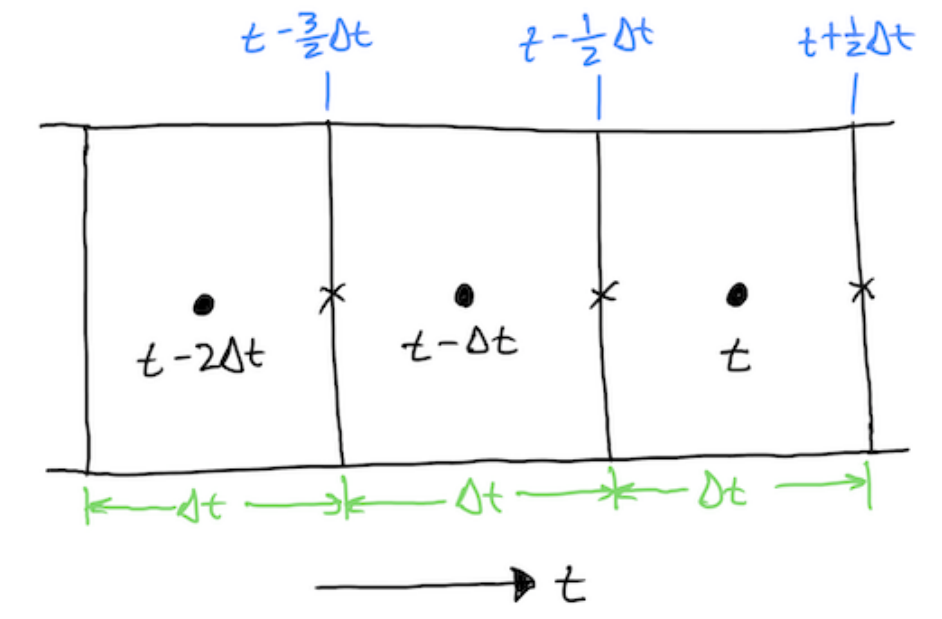
\includegraphics[scale=0.3]{pic/cv_2nd_order_implicit.png}
\end{center}
By using the space-time control volume, the RHS of the discretized equation evaluated at time \(t\), can be considered as a
\uline{representative of the entire timesweep}. The advantages are:
\begin{itemize}
\item we do not need to assume a profile in time, e.g. piecewise constant for fully implicit/explicit, piecewise linear for Crank-Nicholson.
\item no need to store old flux value
\item interpolation depends on the face values:
\begin{itemize}
\item if piecewise constant \(\rightarrow\) 1st order scheme
\item if piecewise linear \(\rightarrow\) 2nd order scheme
\end{itemize}
\end{itemize}
\subsubsection{Derivation}
\label{sec:orgd806b2f}
Integrate the governing equation over the space-time control volume 
\begin{equation}
\int_{t-\Delta t/2}^{t+\Delta t/2} \int_{V} \frac{(\partial \rho c_p T)}{\partial t} dt dV =
\int_{t-\Delta t/2}^{t+\Delta t/2} \int_{V} k \nabla^2 T dt dV + \int_{t-\Delta t/2}^{t+\Delta t/2} \int_{V} S dt dV
\end{equation}
Resulting in:
\begin{equation}
(\rho c_p T_p V_p)^{t+\Delta t/2} - (\rho c_p T_p V_p)^{t-\Delta t/2} = [F_w^d-F_e^d]^t \Delta t + S_P^t \Delta t V_P
\end{equation}
Divide by \(\Delta t\), express the diffusive fluxes in terms of \(D_w\) and \(D_e\), dropping superscripts \(t\) for current time:
\begin{equation}
\frac{(\rho c_p T_P V_P)^{t+\Delta t /2 } - (\rho c_p T_P V_P)^{t-\Delta t /2 }  }{\Delta t} = -D_w (T_P-T_W)
+ D_e (T_E - T_P) + S_P V_P
\end{equation}
LHS is known, for RHS \(\rightarrow\) need to specify values for times \$t-\(\Delta\) t/2 and \(t+\Delta t /2\)
\begin{itemize}
\item 1st order time integration scheme
We assume a \textbf{piecewise constant} distribution over each timestep between the face values, resulting in:
\begin{align*}
T_P^{t-\Delta t /2 } &= T_P^{t-\Delta t }\\
T_P^{t+\Delta t /2 } &= T_P^{t}
\end{align*}
\item 2nd order time integration scheme
We assume a \textbf{piecewise linear} distribution over each timestep between the face values, resulting in:
\begin{align*}
T_P^{t-\Delta t /2} &= T_P^{t-\Delta t } + \frac{1}{2}(T_P^{t-\Delta t} - T_P^{t-2\Delta t})\\
T_P^{t+\Delta t /2} &= T_P^{t} + \frac{1}{2}(T_P^{t} - T_P^{t-\Delta t})\\
\end{align*}
This is achieved by doing backward interpolation and then forward interpolation on the face values.
The schematic below shows these interpolations:
\begin{center}
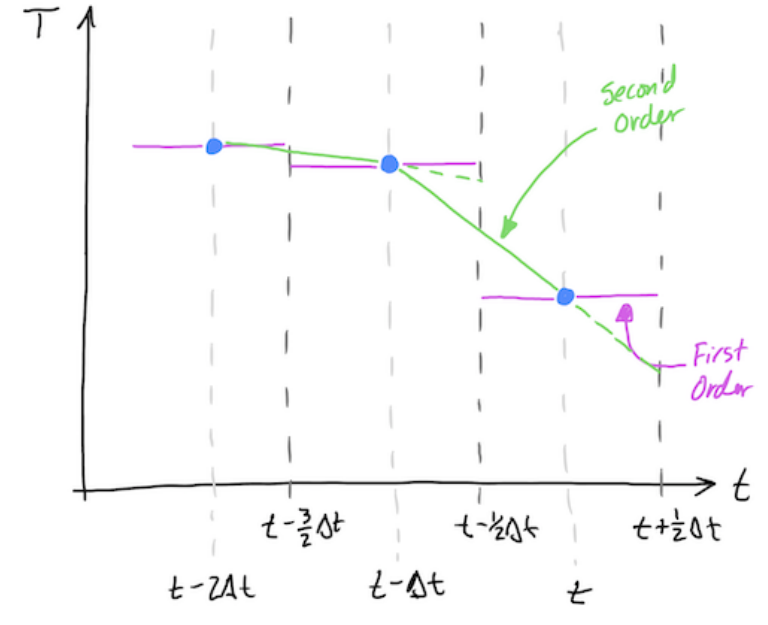
\includegraphics[scale=0.5]{pic/2nd_order_implicit_interpolation.png}
\end{center}
Substituting these relations to the integrated governing equation's LHS:
\begin{itemize}
\item For 1st order scheme:
\begin{equation}
\frac{(\rho c_p T_P V_P)^{t+\Delta t /2} - (\rho c_p T_P V_P)^{t-\Delta t /2 }}{\Delta t} = \rho c_p V_P \frac{T_P - T_P^o}{\Delta t}
\end{equation}
\uline{Note}:
\begin{itemize}
\item the superscript for current time is dropped, and superscript for \(t-\Delta t\) is replaced by \uline{\(o\)} for "old value".
\item also that this is exactly the same as the result for the fully implicit scheme.
\end{itemize}
\item For 2nd order scheme:
\begin{equation*}
\frac{(\rho c_p T_P V_P)^{t+\Delta t /2} - (\rho c_p T_P V_P)^{t-\Delta t /2 }}{\Delta t} =
\rho c_p V_P \frac{T_P + \frac{1}{2}(T_P - T_P^o) - T_P^o - \frac{1}{2}(T_P^o-T_P^{oo})}{\Delta t}
\end{equation*}
or a more simplified version\ldots{}.
\begin{equation}
\frac{(\rho c_p T_P V_P)^{t+\Delta t /2} - (\rho c_p T_P V_P)^{t-\Delta t /2 }}{\Delta t} =
\rho c_p V_P \frac{\frac{3}{2}T_P -2T_P^o + \frac{1}{2}T_P^{oo}}{\Delta t}
\end{equation}
\uline{Note}:
\begin{itemize}
\item superscript \uline{\(oo\)} is used for time value \(t-2\Delta t\).
\item unlike Crank-Nicholson's, flux values at previous timestep \textbf{do not need to be solved}.
Instead, only temperature values at the \textbf{previous two time step} need to be retained.
\end{itemize}
\end{itemize}
\end{itemize}
\subsubsection{Other Transient Discretization Schemes}
\label{sec:org03c5d65}
Some higher order schemes are also used such as:
\begin{itemize}
\item Adams-Bashforth (explicit)
\item Adams-Moulton (implicit)
\item Runge-Kutta (implicit or explicit)
\end{itemize}
\subsubsection{Linearization}
\label{sec:org2083180}
Recall the cell residual for steady conduction:
\begin{equation*}
r_P = D_w (T_P - T_W) - D_e (T_E - T_P) - S_PV_P
\end{equation*}
where \(D_e = \frac{kA_e}{\Delta x_{PE}}\), and \(D_w = \frac{kA_w}{\Delta x_{WP}}\).
If we apply 1st order implicit to the transient term:
\begin{equation*}
r_P = \rho c_p V_P \frac{T_P-T_P^o}{\Delta t}D_w (T_P - T_W) - D_e (T_E - T_P) - S_PV_P
\end{equation*}
This makes the linearization coefficients to be as follow:
\begin{align*}
a_P &= \frac{\partial r_P}{\partial T_P} = \frac{\rho c_p V_P}{\Delta t} + D_w + D_e - \frac{\partial S_P}{\partial T_P}V_P\\
a_W &= \frac{\partial r_P}{\partial T_W} = -D_w\\
a_E &= \frac{\partial r_P}{\partial T_E} = -D_e  
\end{align*}
Similar to before, we can form an algebraic equation for each control volume like this:
\begin{equation}
a_P\delta T_P + a_W\delta T_W + a_E \delta T_E = -r_P 
\end{equation}
If we apply 2nd order implicit temporal scheme instead, then \(a_P\) term would look like this:
\begin{equation*}
a_P = \frac{\partial r_P}{\partial T_P} = \frac{3}{2}\frac{\rho c_p V_P}{\Delta t} + D_w + D_e - \frac{\partial S_P}{\partial T_P}V_P
\end{equation*}
\subsection{Implementation: \href{1d\_heat\_diffusion\_transient.py}{Python code}}
\label{sec:orgdd2220b}
\lstinputlisting[language=Python]{1d_heat_diffusion_transient.py}
\clearpage
\section{ONE-DIMENSIONAL CONVECTION OF A SCALAR}
\label{sec:org0226d77}
\subsection{Problem Definition}
\label{sec:orga394b2f}
For thermal convection, we need the advection-diffusion equation. So far, we only dealt with diffusion, now we add
the advection term which results in:
\begin{equation}
\frac{\partial (\rho c_p T)}{\partial t} + \nabla \cdot (\rho c_p \textbf{u}T) = k \nabla^2 T + S
\end{equation}
assuming constant \(\rho\) and \(c_p\). We also assume that the flow field \(\textbf{u}\) is known,
and we only use it to advect and solve for the temperature field. To preserve continuity across cells, we also
define a mass conservation equation without mass source.
\begin{equation}
\frac{\partial \rho}{\partial t} + \nabla \cdot (\rho \textbf{u}) = 0
\end{equation}
\subsection{Discretization}
\label{sec:org9e7fda4}
Just like we did before, we now integrate the advection-diffusion equation through space and time:
\begin{equation}
\int_{t_0}^{t_1} \int_V \frac{\partial (\rho c_p T)}{\partial t}dtdV + \int_{t_0}^{t_1} \int_V \nabla \cdot (\rho c_p \textbf{u}T)dtdV
= \int_{t_0}^{t_1} \int_V k \nabla^2 T dVdt + \int_{t_0}^{t_1} \int_V SdVdt
\end{equation}
Integration of the transient diffusion equation is covered. Here, we deal with the advection term.
Using the Gauss' divergence theorem to convert volume integral to surface integral:
\begin{equation}
\int_V \nabla \cdot (\rho c_p \textbf{u}T)dV = \int_S (\rho c_p \textbf{u}T)\cdot \textbf{n}dS
\end{equation}
The surface integral is then approximated as discrete sum over the integration points
\begin{equation}
\int_S (\rho c_p \textbf{u}T)\cdot \textbf{n}dS = \sum_{i = 0}^{N_{ip}-1} (\rho c_p \textbf{u}T) \cdot \textbf{n}_{ip} \textbf{A}_{ip}
\end{equation}
For 1D flow across control volume \(P\), this results in:
\begin{equation}
\sum_{i = 0}^{N_{ip}-1} (\rho c_p \textbf{u}T) \cdot \textbf{n}_{ip} \textbf{A}_{ip} = \rho c_p u_e T_e A_e - \rho c_p u_w T_w A_w
\end{equation}
Or in terms of the mass flux, \(\dot{m} = \rho u A\):
\begin{equation}
\sum_{i = 0}^{N_{ip}-1} (\rho c_p \textbf{u}T) \cdot \textbf{n}_{ip} \textbf{A}_{ip} = \dot{m}_e c_p T_e  - \dot{m}_w c_p T_w 
\end{equation}
Note how the \(c_p T\) terms are similar to some forms of internal energy (enthalpy). Thus, we can think off the above equation as the difference
in energy between 2 parcels of fluids, one with internal energy \(c_p T_e\) and one with internal energy \(c_p T_w\)
\begin{center}
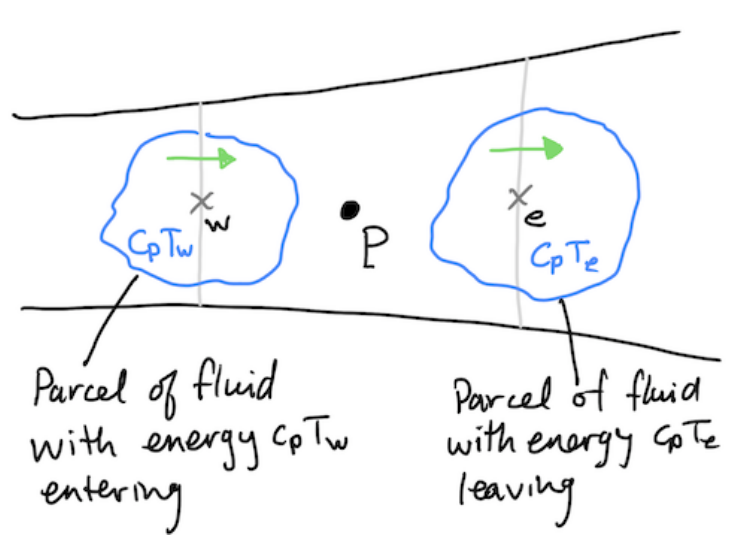
\includegraphics[scale=0.3]{pic/advection_diffusion_parcel.png}
\end{center}
As a result, our discretized energy equation becomes:
\begin{equation}
\begin{aligned}
&\frac{(\rho c_p T_P V_P)^{t+\Delta t /2 } - (\rho c_p T_P V_P)^{t-\Delta t /2}}{\Delta t}  + \dot{m}_e c_p T_e - \dot{m}_w c_p T_w\\
&= -D_w (T_P-T_W) + D_e(T_E-T_P) + S_P V_P
\end{aligned}
\end{equation}
\uline{Note}:
\begin{itemize}
\item transient term is like before, evaluated at time \(t + \Delta t/2\) and \(t - \Delta t/2\).
\item our discretization scheme is \textbf{NOT} completed, because we still do not know how to calculate mass flux and temperature
at integration points, namely \(\dot{m}_e, \dot{m}_w\) and \(T_e, T_w\).
\item we must consider whether the given equation is independent of temperature level according to Rule 4. One can say that it has to
be independent because transient, diffusion, advection terms involve only derivative of temperature. This is true, if mass is conserved
(\(\dot{m}_e = \dot{m}_w\)).  For 1D, this is easy to ensure. For multidimensional problems, this is difficult. In other words, we cannot
assure that the numerical mass fluxes will always be conserved. This can lead to major problem, because if mass is not conserved, one
may think that there is an energy source (or sink) within the domain.
\item to get around the mass conservation problem, we substract the discretized mass equation from the energy equation. Assuming constant density:
\begin{equation*}
\dot{m}_e - \dot{m}_w = 0
\end{equation*}
multiply this by \(T_P\) and \(C_P\) and subtracting from the discretized equation:
\begin{equation}
\begin{aligned}
&\frac{(\rho c_p T_P V_P)^{t+\Delta t /2 } - (\rho c_p T_P V_P)^{t-\Delta t /2}}{\Delta t} + \dot{m}_e c_p (T_e-T_P) - \dot{m}_w c_p (T_w-T_P)\\
&= -D_w (T_P-T_W) + D_e(T_E-T_P) + S_P V_P
\end{aligned}
\end{equation}
This means that if there is a positive imbalance of mass (\(\dot{m_e} > \dot{m}_w\)), there will be a negative source in the energy equation
to counter balance. If there is a negative imbalance, the opposite is true. This step helps with the stability of the numerical method such that
the equations are again independent of the temperature level.
\end{itemize}

\subsection{Advection term with Explicit Time Integration}
\label{sec:orgb41ae7d}
Assume we can interpolate the integration point values in the advection term using a piecewise linear approximation:
\begin{align*}
T_e &= \frac{1}{2}(T_P+T_E)\\
T_w &= \frac{1}{2}(T_W+T_P)
\end{align*}
Assuming no source term and use an explicit time integration scheme, and keeping the \(T_P\) term arising from subtracting the
mass conservation from the energy equation as implicit (i.e. at current timestep). We get the following discretized equation:
\begin{equation*}
\begin{aligned}
\frac{\rho c_p V_P (T_P-T_P^o)}{\Delta t} + &\dot{m}_e c_p \left[\frac{1}{2}(T_P^o+T_E^o) - T_P \right] - \dot{m}_w c_p \left[\frac{1}{2}(T_W^o+T_P^o) - T_P \right]\\
&= -D_w(T_P^o-T_W^o) + D_e(T_E^o-T_P^o)
\end{aligned}
\end{equation*}
where \('o'\) denotes values at previous timestep, and those without superscripts are for current timestep (i.e. those being solved).
We can then group the terms according to their temperature:
\begin{equation*}
\begin{aligned}
\left(  \frac{\rho c_p V_P}{\Delta t} + c_p \dot{m}_w - c_p \dot{m}_e \right  )T_P
&= \left( \frac{\rho c_p V_P}{\Delta t} + \frac{c_p \dot{m}_w}{2} - \frac{c_p \dot{m}_e}{2} -D_e -D_w \right) T_p^o\\
&+\left(D_e - \frac{c_p \dot{m}_e}{2}  \right)T_E^o  +\left(D_w - \frac{c_p \dot{m}_w}{2}  \right)T_W^o
\end{aligned}
\end{equation*}
If mass is conserved, i.e. \(\dot{m}_e = \dot{m}_w\), then:
\begin{equation*}
\begin{aligned}
\frac{\rho c_p V_P}{\Delta t}T_P - &\left( \frac{\rho c_p V_P}{\Delta t} -D_e -D_w \right) T_p^o - \left(D_e - \frac{c_p \dot{m}_e}{2}  \right)T_E^o\\
&+\left(D_w - \frac{c_p \dot{m}_w}{2}  \right)T_W^o = 0
\end{aligned}
\end{equation*}
From Rule 2, we need :
\begin{itemize}
\item the coefficient on \(T_P\) to be \uline{positive\_}
\item the coefficients on remaining terms, \(T_P^o\), \(T_E^o\), and \(T_W^o\) to be \uline{negative}.
\end{itemize}
For \(T_P^o\), this requires:
\begin{equation*}
D_e + D_w \leq \frac{\rho c_p V_P}{\Delta t}
\end{equation*}
or:
\begin{equation*}
\Delta t \leq \frac{\rho c_p V_P}{D_e + D_w}
\end{equation*}
Refer to chapter 3, we see that this is the same timestep restriction in the form:
\begin{equation*}
\boxed{\frac{\alpha \Delta t}{\Delta x^2} \leq \frac{1}{2}}
\end{equation*}
where \(\alpha = \frac{k}{\rho c_p}\). We can say that the addition of the advection term does not change the timestep restriction.
Note how the coefficients for \(T_P^o\) and \(T_E^o\) \textbf{can be positive} for certain mass flow rates. Thus, for \(T_E^o\), we need the following
condition:
\begin{equation*}
D_e \geq \frac{c_p \dot{m}_e}{2}
\end{equation*}
simplifying\ldots{}
\begin{equation*}
\begin{aligned}
D_e & \geq \frac{c_p \dot{m}_e}{2}\\
\frac{kA}{\Delta x} & \geq \frac{c_p \rho u A}{2}\\
\Delta x &\leq \frac{2k}{\rho c_p u}
\end{aligned}
\end{equation*}
or in terms of the thermal diffusivity, \(\alpha\):
\begin{equation*}
\boxed{\frac{u \Delta x}{\alpha} < 2 }
\end{equation*}
To sum up, we have both the spatial and temporal conditions on \(\Delta x\) and \(\Delta t\). Multiplying them together:
\begin{equation*}
\begin{aligned}
\frac{\alpha \Delta t}{\Delta x^2}\cdot \frac{u \Delta x}{\alpha} &< \frac{1}{2}\cdot 2\\
\frac{u \Delta t}{\Delta x} &< 1
\end{aligned}
\end{equation*}
The LHS is known as the Courant number, thus the space-time restriction can be written as:
\begin{equation}
\boxed{Co < 1}
\end{equation}
To see whether such restriction is serious. \\
Consider flow in a tube with constant wall temperature, \(T_w\), this problem has the exact solution as:
\begin{equation*}
\frac{T_w - T(x)}{T_w=T_{in}} = exp\left(-\frac{hP}{\dot{m}c_p}x \right)
\end{equation*}
\begin{center}
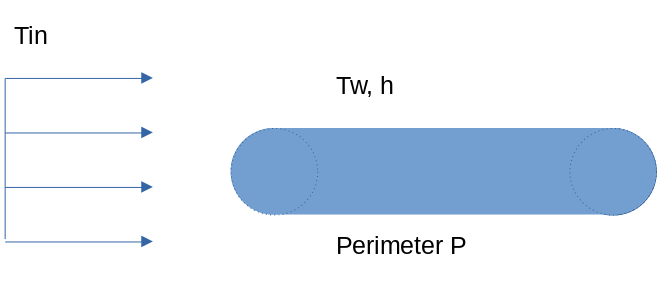
\includegraphics[scale=0.5]{pic/tube_twall.png}
\end{center}
Let us consider the solution for this problem unil some point \(x_L\) where the bulk temperature difference, \((T_w - T(x))\)
reached \(5\%\) the difference in inlet and wall, \((T_w-T_{in})\), i.e.
\begin{equation*}
\frac{T_w-T(x_L)}{T_w-T_{in}} = 0.05
\end{equation*}
We further assume the Nusselt number is defined as:
\begin{equation*}
Nu = \frac{hD}{k}
\end{equation*}
Then the general solution for this particular geomtry is as follow:
\begin{equation*}
\frac{T_w - T(x)}{T_w=T_{in}} = exp\left(  -\frac{   \frac{Nuk}{D} \pi D } {\rho u \pi \frac{D^2}{4}  c_p} x_L \right) = exp\left(- \frac{4Nu\alpha}{uD^2}x_L   \right)
\end{equation*}
By definition, \(uD/\alpha = RePr\), \(R_e = uD/\nu\) and \(Pr = \nu/\alpha\):
\begin{equation*}
\frac{T_w - T(x)}{T_w=T_{in}} = exp\left(- \frac{4Nu}{RePr}\frac{x_L}{D}   \right)
\end{equation*}
Recall we want \(5\%\) between the temperature difference
\begin{equation*}
\begin{aligned}
\frac{4Nu}{RePr}\frac{x_L}{D} &= 3\\
\frac{x_L}{D} &= \frac{3}{4}\frac{RePr}{Nu}
\end{aligned}
\end{equation*}
Now, we use the restriction from above, \(\Delta x \leq 2\alpha / u\) and the definition of the number of control volume, \(N_{cv} = x_L/\Delta x\):
\begin{equation*}
\boxed{N_{cv} \leq \frac{x_L}{\Delta x} = \frac{3}{8}\frac{Re^2Pr^2}{Nu}}
\end{equation*}
Using some numbers to test:
\begin{center}
\begin{tabular}{ll}
\textbf{PARAMETERS} & \textbf{NO. OF CONTROL VOLUME}\\
\hline
 & \\
Nu = 5, Re = 1000, Pr = 1 & \(10^5\) = 100,000\\
Nu = 5, Re = 1000, Pr = 10 & \(10^7\) = 10,000,000\\
\end{tabular}
\end{center}
\uline{Note}: a 10 times increase in Pr results in \(10^7\) number of control volume. This is impractical because it means that we need to solve
\(10^7\) equations. So what is the required minimum number of timestep? We can calculate this by taking the ratio between \uline{the time it take for a fluid
to exit the pipe} to the \uline{time step restriction we derived above}:
\begin{equation*}
\begin{aligned}
N_t &= \frac{x_L/u}{\Delta t}\\
&= \frac{\frac{3}{4}\frac{RePr}{Nu}\frac{D}{u}}{\frac{1}{2}\frac{\Delta x^2}{\alpha}}\\
&= \frac{3}{8}\frac{Re^2Pr^2}{Nu}
\end{aligned}
\end{equation*}
Again, using some numbers, we face similar problem: too impractical. 
\begin{center}
\begin{tabular}{ll}
\textbf{PARAMETERS} & \textbf{NO. OF CONTROL VOLUME}\\
\hline
 & \\
Nu = 5, Re = 1000, Pr = 1 & \(10^5\) = 100,000\\
Nu = 5, Re = 1000, Pr = 10 & \(10^7\) = 10,000,000\\
\end{tabular}
\end{center}
Next, we will discuss in more details about these restrictions. 

\subsection{Discussion of the Restrictions on Timestep}
\label{sec:org9bda366}
We see how explicit scheme results in timestep restriction.
Next, let's consider a 1st order implicit scheme:
\begin{equation*}
\begin{aligned}
&\left(  \frac{\rho c_p V_P}{\Delta t} + D_e + D_w + c_p \dot{m}_w - c_p \dot{m}_e \right  )T_P
- \left( D_e - \frac{c_p \dot{m}_e}{2} \right) T_E\\
&-\left(D_w + \frac{c_p \dot{m}_e}{2}  \right)T_W  - \frac{\rho c_p V_p}{\Delta t}T_P^o = 0
\end{aligned}
\end{equation*}
Rule 2 requires coefficient on \(T_p\) to be \uline{positive}. From above equation, there is no time restriction because coefficient on \(T_p\) is always positive, assuming mass is conserved.\\
On the other hand, \(T_W\) and \(T_E\) ' coefficients need to be \uline{negative}:
\begin{equation*}
\begin{aligned}
D_e - \frac{c_p \dot{m}_e}{2} &\leq 0\\
\frac{u \Delta x}{\alpha} &\leq 2
\end{aligned}
\end{equation*}
Previous analysis still applies so the number of control volume is still large (even if there is no restriction on the timestep size)

\subsection{Discussion of the Restriction on Spatial Resolution}
\label{sec:org0bc4bb0}
By moving to an implicit time integration scheme, we encountered restriction on time step. \\
Follow the same logic, we can also say that the restriction on grid size must come from the interpolation method chosen
for the integration point in the advection term.\\
Again, we consider flow in a duct where analytical solution is known and can be applied between \(P\) and \(E\) locations.
Our temperature profile between cell centers is:
\begin{equation*}
\frac{T-T_P}{T_E-T_P} = \frac{\textrm{exp}\left[Pe_\Delta \left(\frac{x-x_P}{x-x_P}  \right)       \right] -1 }
{\textrm{exp}(Pe_\Delta)-1}
\end{equation*}
where \(Pe_\Delta\) is the Pectet number representing ratio of convection to diffusion
\begin{equation*}
\begin{aligned}
Pe_\Delta &= \frac{u \Delta x}{\alpha}\\
&=  \frac{u \Delta x}{\alpha} \cdot \frac{\mu / \rho}{\mu / \rho}\\
&= \frac{(\mu / \rho) u \Delta x}{(\mu / \rho)\alpha}\\
&= \frac{\nu}{\alpha}\left(\frac{u \Delta x}{\mu / \rho}\right)\\
&= \frac{\nu}{\alpha}\left(\frac{ \rho u \Delta x}{\mu}\right)\\
&= Re_\Delta Pr
\end{aligned}
\end{equation*}
with the following flow regimes:
\begin{itemize}
\item \(Pe_\Delta \approx 0\): diffusion dominates
\item \(|Pe_\Delta| \approx 1\): convection and diffusion
\item \(|Pe_\Delta| \gg 1\): convection dominates
\end{itemize}
Visualization for different values of \(Pe_\Delta\): \href{pectet\_visualize\_pipe.py}{Python code}
\lstinputlisting[language=Python]{pectet_visualize_pipe.py}

\begin{center}
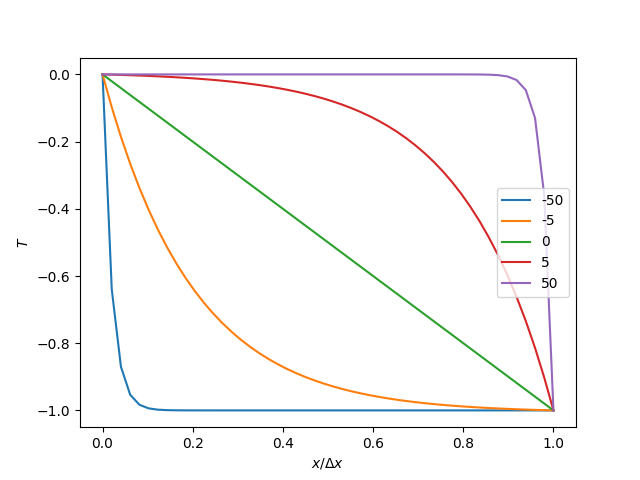
\includegraphics[scale=0.8]{pic/pectet_visual_pipe.png}
\end{center}
We note from the figure above that our assumption piecewise linear temperature profile, using
the \uline{central difference scheme (CDS)}, is only valid for \(Pe_\Delta \approx 0\). \\
In practice, \(Pe_\Delta\) will be large and thus we need different interpolation scheme. 

\subsection{The Upwind Difference Scheme (UDS)}
\label{sec:org332b529}
We attempt a new interpolation scheme, upwind difference scheme. For the east integration point, we have:
\begin{equation}
T_e = \frac{1+\alpha _e}{2} T_P + \frac{1-\alpha_e}{2}T_E
\end{equation}
with \(\alpha\) being the weighting factor, i.e.
\begin{itemize}
\item \(Pe_\Delta \approx 0\) , \(\alpha_e = 0\) : diffusion dominates, CDS recovered
\item \(|Pe_\Delta| \approx 1\), \(\alpha_e = 1\) : convection and diffusion, \(T_e = T_P\)
\item \(|Pe_\Delta| \gg 1\), \(\alpha_e = -1\): convection dominates, \(T_e = T_E\)
\end{itemize}
Using this new interpolation scheme, the discrete equation in terms of the cell residual becomes:
\begin{equation*}
\begin{aligned}
r_P &= \left(\frac{\rho c_p v_P}{\Delta t}+D_e + D_w + \frac{1}{2}c_p\dot{m}_w(1+\alpha_w) - \frac{1}{2}c_p\dot{m}_e(1-\alpha_e) \right)T_P\\
-&\left[D_e -\frac{1}{2}c_p\dot{m}_e(1-\alpha_e)\right]T_E - \left[D_w +\frac{1}{2}c_p\dot{m}_w(1+\alpha_w)\right]T_W
- \frac{\rho c_p V_P}{\Delta t} T_P^o
\end{aligned}
\end{equation*}
with the following linearization coefficients:
\begin{equation}
\begin{aligned}
a_W &= -D_w - \frac{1}{2}c_p \dot{m}w(1+\alpha_w)\\
a_E &= -D_e + \frac{1}{2}c_p \dot{m}_e(1-\alpha_e)\\
a_P &= \frac{\rho c_p v_P}{\Delta t} - a_W - a_E
\end{aligned}
\end{equation}
For fast flowing fluid in the positive direction, \(\alpha_w = \alpha_e = 1\). Our east/west coefficients become:
\begin{equation*}
\begin{aligned}
a_W &= -D_e - c_p \dot{m}w\\
a_E &= D_e
\end{aligned}
\end{equation*}
To satisfy Rule 2, here the coefficients cannot become positive, because the fluid is flowing in the positive direction
and \(\dot{m}_w\) is positive. In contrast, for a fluid flowing in the negative direction, \$\(\alpha\)\textsubscript{w} = \(\alpha\)\textsubscript{e} = -1 \$ and
the coefficients become:
\begin{equation*}
\begin{aligned}
a_W &= -D_w\\
a_E &= -D_e + c_p \dot{m}e
\end{aligned}
\end{equation*}
Again, these cannot be positive because \(\dot{m}_e\) is negative in this case. As a result, we can see that using Upwind Difference
Scheme ensures the solution is stable for any \(\Delta x\). Combining this with an implicit time integration scheme means that
there are no formal restrictions on timestep or grid size. 

\subsection{False Diffusion}
\label{sec:org9d97b37}
UDS is only 1st order and only when \(\alpha_e = \pm 1\). Here, we try to estimate the accuracy of UDS against CDS
using Taylor series about east face integration point.
\begin{center}
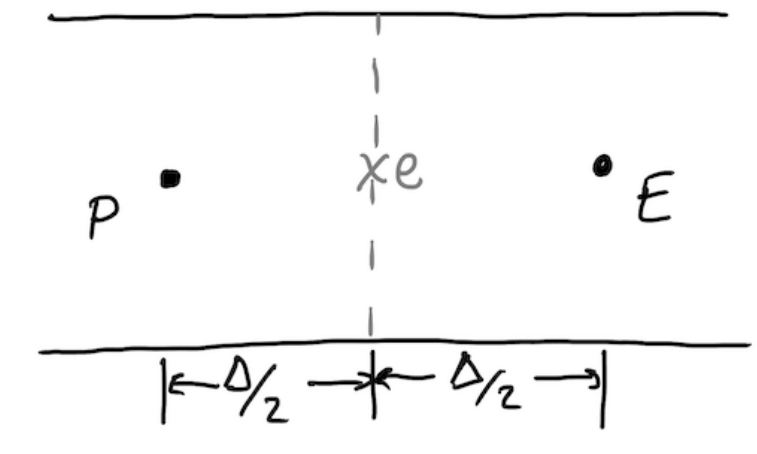
\includegraphics[scale=0.5]{pic/false_diffusion.png}
\end{center}
Expanding about this point gives the following cell values:
\begin{equation*}
\begin{aligned}
T_E &= T_e + \frac{\Delta}{2}{dT}{dx}\biggr \rvert_e + \frac{(\Delta / 2)^2}{2}\frac{d^2T}{dx^2}\biggr \rvert_e + ... \\
T_P &= T_e - \frac{\Delta}{2}{dT}{dx}\biggr \rvert_e + \frac{(\Delta / 2)^2}{2}\frac{d^2T}{dx^2}\biggr \rvert_e - ... 
\end{aligned}
\end{equation*}
Recall the CDS interpolation, \(T_e = 1/2(T_P + T_E)\). We sub this into the above estimates:
\begin{equation*}
T_e^{CDS} = T_e + \frac{(\Delta / 2)^2}{2}\frac{d^2 T}{dx^2}\biggr \rvert _e + O(\Delta ^4)
\end{equation*}
Likewise, for UDS, we assume flow in the positive direction:
\begin{equation}
T_e^{UDS} = T_P = T_e - \frac{\Delta}{2}\frac{dT}{dx}\biggr \rvert _e + O(\Delta ^2)
\end{equation}
The error is based on the first truncated term. For both cases (UDS and CDS), the leading term is \(T_e\) and the next term
is the truncated term.
\begin{equation*}
\begin{aligned}
e^{CDS} &\sim \dot{m}c_p \frac{(\Delta / 2)^2}{2}\frac{d^2T}{dx^2} \biggr \rvert_e \sim O(\Delta ^2)\\
e^{UDS} &\sim \dot{m}c_p \frac{\Delta}{2}\frac{dT}{dx}\biggr \rvert _e \sim O(\Delta)
\end{aligned}
\end{equation*}
Note how we have the \(\dot{m}c_p\) term, this is because the integration point temperatures are multiplied by this value in
the energy equation. Thus, this is the full error for that term, not just the error for the interpolated values. We can conclude
that CDS is 2nd order accurate in space, while UDS is only 1st order in space. Another way to think is: if we half the grid size,
the UDS error will reduce by factor of 2, while the CDS will reduce by factor of 4.\\
Note also that the error for UDS is proportional to the temperature gradient in the energy equation, this behaves very much like
a diffusion term: \(k\frac{dT}{dx}\). We call this `false diffusion'.
\begin{equation*}
e^{UDS} = -\dot{m}c_p \frac{\Delta}{2}\frac{dT}{dx}\biggr \rvert_e = -\frac{\rho c_p u_e A_e \Delta}{2}\frac{dT}{dx}\biggr\rvert_e
= -\Gamma^{false}\frac{dT}{dx}\biggr\rvert_e A_e
\end{equation*}
with \(\Gamma^{false} = \frac{\rho c_p u_e \Delta}{2}\). Obviously, our real diffusion involves \(k\) and \(\nabla T\). Taking the ratio
between these:
\begin{equation*}
\begin{aligned}
\frac{\Gamma^{false}}{\Gamma^{real}} = \frac{\rho c_p u_e \Delta}{2k} = \frac{1}{2}\frac{u\Delta}{\nu}\frac{\nu \rho c_p }{k}
= \frac{1}{2}\frac{u\Delta}{\nu}\frac{\nu}{\alpha} = \frac{1}{2}Re_\Delta Pr = \frac{1}{2}Pe_\Delta
\end{aligned}
\end{equation*}
\uline{Note}: for large \(Pe\), false diffusion dominates real diffusion. This is bad because we can't model real diffusion. However,
note that in our analysis, we assume that the \texttt{leading term} is a good estimation of the error. For convection problem, this may
not be the case. To test this, let us consider the exact solution between points \(P\) and \(E\):
\begin{equation*}
\frac{T-T_p}{T_E-T_P} = \frac{\textrm{exp}(Pe (x^*))-1}{\textrm{exp}(Pe)-1}
\end{equation*}
where:
\begin{equation*}
\begin{aligned}
Pe &= Pe_\Delta\\
x^* &= \left( \frac{x-x_P}{x_E-x_P} \right)
\end{aligned}
\end{equation*}
or we can think of it like this:
\begin{equation*}
T-T_p =(T_E-T_P) \frac{\textrm{exp}(Pe (x^*))-1}{\textrm{exp}(Pe)-1} = A[\textrm{exp}(Pe (x^*))-1]
\end{equation*}
Recall the Taylor series expansion for \(T_P\) up to 4 terms is:
\begin{equation*}
T_P = T_e - \frac{\Delta}{2}\frac{dT}{dx}\biggr \rvert_e + \frac{(\Delta / 2)^2}{2}\frac{d^2T}{dx^2}\biggr \rvert_e -
\frac{(\Delta / 2)^3}{6}\frac{d^3T}{dx^3}\biggr \rvert_e 
\end{equation*}
The first derivative term in the Taylor series, for this particular solution is:
\begin{equation*}
\begin{aligned}
\frac{dT}{dx}\biggr\rvert_e &= \frac{dT}{dx^*}\biggr\rvert_e \frac{dx^*}{dx}\\
\frac{dx^*}{dx} &= \frac{1}{x_E-x_P} = \frac{1}{\Delta}\\
\frac{dT}{dx^*}\biggr \rvert_e &= APe\textrm{ exp}(Pe (x&*)) = APe\textrm{ exp}\left(\frac{Pe}{2}\right)
\end{aligned}
\end{equation*}
Following the same procedure, we can find out expressions for the 2nd and 3rd derivatives. Plugging into the Taylor series for T\(T_P\):
\begin{equation*}
T_P = ... = T_e - \frac{APe \textrm{ exp} \left(\frac{Pe}{2}\right)} {2} \left[1 - \frac{Pe}{4} + \frac{Pe}{24} \right]
\end{equation*}
Let:
\begin{equation*}
S = \left[1 - \frac{Pe}{4} + \frac{Pe}{24} \right]
\end{equation*}
\end{document}